% Transportation Research Board conference paper template
% version 1.1
% 
% David R. Pritchard, http://davidpritchard.org
%   1.0 - Mar. 2009
%   1.1 - Sep. 2011, fixes for captions

% PAGE LAYOUT
%------------------------------------------

% Custom paper settings...
\documentclass[titlepage,oneside,12pt]{article}

\oddsidemargin 0.0in
\topmargin -0.5in
\headheight 0.3in
\headsep 0.2in
\textwidth 6.5in
\textheight 9.0in
\setlength{\parindent}{0.5in}

\usepackage{hyperref}

% PAGE HEADER
%------------------------------------------
% Adjust the header text below (INSERT AUTHORS HERE)
\oddsidemargin 0.0in
\usepackage{lscape}
\usepackage[tiny,rm]{titlesec}
\usepackage{titling}
\usepackage{xcolor}
\newpagestyle{trbstyle}{
	\sethead{Apostolov and Oke}{}{\thepage}
}
\pagestyle{trbstyle}

% HEADINGS
%------------------------------------------
\titleformat{\section}{\bfseries}{}{0pt}{\uppercase}
\titlespacing*{\section}{0pt}{12pt}{*0}
\titleformat{\subsection}{\bfseries}{}{0pt}{}
\titlespacing*{\subsection}{0pt}{12pt}{*0}
\titleformat{\subsubsection}{\itshape}{}{0pt}{}
\titlespacing*{\subsubsection}{0pt}{12pt}{*0}

% LISTS
%------------------------------------------
% Adjust lists a little. Not quite perfectly fitting TRB style, but vaguely
% close at least.
%\usepackage{enumitem}
%\setlist[1]{labelindent=0.5in,leftmargin=*}
%\setlist[2]{labelindent=0in,leftmargin=*}

\usepackage{booktabs}
% CAPTIONS
%------------------------------------------
% Get the captions right. Authors must still be careful to use "Title Case"
% for table captions, and "Sentence case." for figure captions.
\usepackage{ccaption}
\usepackage{amsmath}
\makeatletter
\renewcommand{\fnum@figure}{\textbf{FIGURE~\thefigure} }
\renewcommand{\fnum@table}{\textbf{TABLE~\thetable} }
\makeatother
\captiontitlefont{\bfseries \boldmath}
\captiondelim{\;}
%\precaption{\boldmath}

% FONTS
%------------------------------------------
% Three options for fonts. I prefer Times for text and Computer Modern for
% math.

% Times for text, Computer Modern for math
\usepackage{times}
% Times for text and math
%\usepackage{pslatex}
% Times for text and math
%\usepackage{times,mathptmx} 

% Some pdf conversion tricks? Unsure.
\usepackage[T1]{fontenc}
\usepackage{textcomp}
\usepackage{bm}
\usepackage{makecell}
\usepackage{subfig}
\def\checkmark{\tikz\fill[scale=0.4](0,.35) -- (.25,0) -- (1,.7) -- (.25,.15) -- cycle;}

% CITATIONS
%------------------------------------------
% TRB uses an Author (num) citation style. I haven't found a way to make
% LaTeX/Bibtex do this automatically using the standard \trbcite macro, but
% this modified \trbcite macro does the trick.

% TODO: sort&compress option?
\usepackage[sort,numbers]{natbib}
\newcommand{\trbcite}[1]{({\it \citenum{#1}})}
\newcommand{\trbcitet}[1]{\citeauthor{#1} ({\it \citenum{#1}})}

\setcitestyle{round}

%% Cite Title
%\usepackage[style=authoryear,backend=biber,natbib,maxcitenames=2,doi=false,isbn=false,url=false,eprint=false]{biblatex}
%\addbibresource{bib/references.bib}

%\usepackage{hyperref}

% LINE NUMBERING
%------------------------------------------
% TRB likes line numbers on drafts to help reviewers refer to parts of the
% document. Comment out for final versions.
\usepackage{lineno}
\renewcommand\linenumberfont{\normalfont\small}
\linenumbers


% COUNTERS
%------------------------------------------
% TRB requires the total number of words, figures, and tables to be displayed on
% the title page. This is possible under the totcount package on CTAN.
\usepackage{totcount}
	\regtotcounter{table} 	%count tables
	\regtotcounter{figure} 	%count figures

\newcommand\wordcount{\immediate\write18{texcount -sum -1 \jobname.tex > 'count.txt'} \input{count.txt} }
  
% DOCUMENT START
%------------------------------------------
% Add any additional \usepackage declarations here.

\usepackage{graphicx}
\graphicspath{{./images/}}
 
\usepackage{rotating}
\usepackage{longtable}

%\usepackage{enumerate}
\usepackage{paralist}

%%%TIKZ
\usepackage{tikz}
\usepackage{pgfplots}
\usepackage{pgfplotstable}
\usepackage{pgfgantt}
\pgfplotsset{compat=newest}

\usetikzlibrary{arrows,shapes,positioning,shapes.geometric}
\usetikzlibrary{decorations.markings}
\usetikzlibrary{shadows,automata}
\usetikzlibrary{patterns}
\usetikzlibrary{trees,mindmap,backgrounds}
%\usetikzlibrary{circuits.ee.IEC}
\usetikzlibrary{decorations.text}
% For Sagnac Picture
\usetikzlibrary{%
    decorations.pathreplacing,%
    decorations.pathmorphing%
}
\tikzset{no shadows/.style={general shadow/.style=}}
%
%\usepackage{paralist}

%%% FORMAT PYTHON CODE
\usepackage{listings}
% Default fixed font does not support bold face
\DeclareFixedFont{\ttb}{T1}{txtt}{bx}{n}{8} % for bold
\DeclareFixedFont{\ttm}{T1}{txtt}{m}{n}{8}  % for normal

% Custom colors
\usepackage{color}
\definecolor{deepblue}{rgb}{0,0,0.5}
\definecolor{deepred}{rgb}{0.6,0,0}
\definecolor{deepgreen}{rgb}{0,0.5,0}

\newcommand{\osn}{\oldstylenums}
\newcommand{\dg}{^{\circ}}
\newcommand{\lt}{\left}
\newcommand{\rt}{\right}
\newcommand{\pt}{\phantom}
\newcommand{\tf}{\therefore}
\newcommand{\?}{\stackrel{?}{=}}
\newcommand{\fr}{\frac}
\newcommand{\dfr}{\dfrac}
\newcommand{\ul}{\underline}
\newcommand{\tn}{\tabularnewline}
\newcommand{\nl}{\newline}
\newcommand\relph[1]{\mathrel{\phantom{#1}}}
\newcommand{\cm}{\checkmark}
\newcommand{\ol}{\overline}
\newcommand{\rd}{\color{red}}
\newcommand{\bl}{\color{blue}}
\newcommand{\pl}{\color{purple}}
\newcommand{\og}{\color{orange!90!black}}
\newcommand{\gr}{\color{green!40!black}}
\newcommand{\nin}{\noindent}
\newcommand{\la}{\lambda}
\renewcommand{\th}{\theta}
\newcommand{\al}{\alpha}
\newcommand{\G}{\Gamma}
\newcommand*\circled[1]{\tikz[baseline=(char.base)]{
            \node[shape=circle,draw,thick,inner sep=1pt] (char) {\small #1};}}

\newcommand{\bc}{\begin{compactenum}[\quad--]}
\newcommand{\ec}{\end{compactenum}}

\newcommand{\p}{\partial}
\newcommand{\pd}[2]{\frac{\partial{#1}}{\partial{#2}}}
\newcommand{\dpd}[2]{\dfrac{\partial{#1}}{\partial{#2}}}
\newcommand{\pdd}[2]{\frac{\partial^2{#1}}{\partial{#2}^2}}

\begin{document}
\renewcommand{\refname}{\uppercase{References}}
% \raggedright

\begin{titlepage}
\begin{flushleft}

% Title
{\LARGE \bfseries Investigating country-level activity and mobility patterns  and their interdependencies on COVID-19 outcomes}\\[1cm]

%%%%%%%%%%%%%%%%%%%%%%%%%%%%%%
%%% Provisional author list; to be finalized once draft is ready.
%%%%%%%%%%%%%%%%%%%%%%%%%%%%%%5

 \textbf{Atanas Apostolov\textsuperscript{1}} \\
 Email: aapostolov@umass.edu  \\[0.5cm]

 \textbf{Jimi B.\ Oke\textsuperscript{1}} \\
 %\textit{Corresponding Author} \\
 Email: jboke@umass.edu  \\[0.5 cm]

% \textbf{Author 3 \textsuperscript{1}} \\
% Email: @ ; Phone: \\[0.5 cm]
 
 
\textbf{\textsuperscript{1} Department of Civil and Environmental Engineering, University of Massachusetts Amherst, MA 01003, United States} \\[0.3 cm]
%\textbf{\textsuperscript{2} Department of Civil and Environmental Engineering, University of Massachusetts Amherst, MA 01003, United States} \\[0.3 cm]


\wordcount words + \total{table} tables %+ \total{figure} figures

\today

\end{flushleft}
\end{titlepage}

%% This generates the title page from the information given above.
\thispagestyle{empty}
%\maketitle

\newpage

\thispagestyle{empty}
 

\section{Abstract}
In this paper we examine the effects of COVID-19 on mobility, segmented by transportation type, as well as social activity such as retail and recreation, workplaces and residential, and their interdependencies.
Using time series data from 63 countries across five continents,
we investigate patterns in activity and mobility trends from January through July.
Our clustering approach yields four clusters of countries with similar behavior.
We plan to estimate vector autoregression models  to analyze the relationship between activity changes, mobility changes and COVID-19 growth.
We will also fit cluster-level models and a global model which includes exogenous variables (such as interventions).
Our findings yield insights into how various activities have been impacted by COVID-19 and vice-versa.
We expect that our model outcomes will guide policymakers to adopt  appropriate  measures to mitigate and safely recover from the ongoing pandemic, as well as future ones.

\section{Introduction}
COVID-19 has had a severe impact on mobility and social activities since initial reports of the disease emerged in late 2019.
By May 2020 most countries had implemented social distancing measures and imposed strict travel restrictions to curtail the spread of the virus
both within their borders and internationally.
According to \trbcite{bonaccorsi2020economic}, the international spread of the disease can be partially explained by risk perception,
mobility behavior and social media influences using a global vector autoregression (GVAR) modeling framework\cite{dees2007exploring}.
%Milani concludes that most countries learn from each other's social distancing response which can be partially explained by social networks.  
\trbcite{zhang2020pathways} confirm that human mobility is key to understanding the transmission pathways.
Using a mobility dataset of over 500,000 flights and over 100 million passengers,
the authors develop a dynamic network model using time-dependent border restrictions as exogenous variables.
\trbcite{mckenzie2020country} studied the patterns in 6 activity responses across 108 countries but this was an exploratory effort in comparison with government policies and it included no modeling attempt to explain COVID-19 outcomes.

Beyond these global studies, several city and country-specific simulations and models have been estimated to explain how activities, mobility (particularly transit) impact COVID-19 outcomes.
\trbcite{kumar2020activitybased} used an activity-based epidemiological framework to study how COVID-19 is propagated across various daily activities in car-dependent cities typically found in the US and Canada.
They quantified the effect of the transit network on COVID-19 spread and demonstrated the importance of work and home activities in the early and latter stages of the epidemic.
\trbcite{badr2020association} developed a generalized linear model to explain COVID-19 growth based on overall mobility changes at the county level in the US. Inter-county movements were factored in but impacts by mode or activity were not analyzed.
Given China's and then  Italy's prominence in the earlier stages of the pandemic, several studies have examined their mobility patterns \trbcite{
  kraemer2020effect,bonaccorsi2020economic,pepe2020covid19,carteni2020how}.
While these have been important for country-wide epidemiological studies, they have not provided knowledge on activity-based impacts.

A study on human mobility across countries aggregates data on a daily basis and uses a dynamic spatial network model to estimate the confirmed infections in each country from a global sample. \trbcite{zhang2020covid19} Passenger flight capacity is used as opposed to the actual number of passengers who flew in the studied time frame (January to April, 2020). According to the results, there is an association between the number of daily new cases in the US and the epidemics in Europe, South America and Africa. Furthermore, there is a mutual correlation among European countries. Aggregated location data is also used in the mobility networks models explaining inequities but focusing solely on the US. 

Therefore, there remains an urgent need to understand the interdependencies between COVID-19 outcomes and human mobility and activity patterns.
Statistically significant models can yield insights to enable policymakers contain and recover from the ongoing pandemic.
Furthermore, these models can guide future decisions in containing the spread of future epidemics.
In this paper, we conduct a global scale country-level analysis of COVID-19 infections,  mobility and activity patterns.
First, we cluster the countries to discover patterns in mobility and activity changes.
Second, we estimate cluster-representative models using the vector autoregression (VAR) framework, allowing for time lags across all endogenous variables, and thus including dynamic interdependencies among them.
These models explain which activities impact COVID-19 outcomes and vice versa, providing potential pathways for understanding behavioral responses to the spread of the pandemic and a greater understanding of the disparities and similarities across nationwide outcomes.

%By assigning a value of zero or one to international mobility restrictions, Zhang et al discover a direct relationship between the transmission rates and the coefficients in the estimation outcome, i.e. positive coefficients indicate effectiveness. 

% \trbcite{forecasting} shed light on forecasting with Bayesian Global Vector Autoregressive Model. This statistical approach pertains to the impacts of mobility on COVID-19 due to its counterfactual nature; instead of treating observations in isolation B-GVAR accommodates variable interdependence and produces more robust forecasts. Country-specific models can be converted to a system of equations where all endogenous variables are stacked. Although taking into account international linkages improves the forecast, the optimal lag for each country still needs to be estimated and tested for stationarity 



\section{Data}
We use transportation data provided by Apple\footnote{\url{https://www.apple.com/covid19/mobility}} along with Community Mobility Reports compiled by Google\footnote{\url{https://www.google.com/covid19/mobility/}}. %The data is publicly available at:
The new confirmed cases global data set is provided by the Johns Hopkins University COVID-19 Data initiative\footnote{\url{https://github.com/CSSEGISandData/COVID-19}}.
Apple's data set focuses on transportation types (walking, driving, transit) whereas Google tracks movement trends by region and segments them into categories such as residential, workplace and transit. Our integrated data set captures changes in requests for directions from January 22 to July 14 as well as aggregated location data for a variety of categorized places. The data shows us the change in visitors from February 15 to July 12 compared to a baseline of days (January 3 - February 6, 2020). By tracking user requests of their Maps application, Apple contributes a snapshot of incidental trips as opposed to actual foot traffic which is the approach taken by Google for their Community Mobility Reports. 
The sources are summarized in \autoref{tab:sources} and the variables are described in \autoref{tab:variables}.
The integrated dataset (along with the code and plots generated for this paper) is publicly available on Github.\footnote{\url{https://github.com/narslab/covid-analysis/tree/master/mobility}}


\begin{table}[h!]\small
  \centering
  \caption{Summary of data sources}
  \label{tab:sources}
\begin{tabular}{ll}\toprule
\bf Source                         & \bf Overview                                                                              \\\midrule
Johns Hopkins University          & Time series summary globally.                                                               \\
Apple Maps                        & Compared to a baseline volume on January 13th, 2020.                                          \\
  Google Community Mobility Reports & Compared to a baseline day \\
  & (median value over period from Jan 3 to Feb 6, 2020)\\\bottomrule
\end{tabular}
\end{table}

\begin{table}[h!]
  \centering
\caption{Summary of variables}
\label{tab:variables}
\small
\begin{tabular}{ll}\toprule
\textbf{Variable}                                         & \textbf{Description}                                    \\\midrule
covid\_cases & New COVID-19 cases as tracked by Johns Hopkins University. \\
retail\_and\_recreation\_percent\_change\_from\_baseline & Retail and recreation movement trends.            \\
grocery\_and\_pharmacy\_percent\_change\_from\_baseline  & Grocery and pharmacy movement trends.             \\
parks\_percent\_change\_from\_baseline                   & Parks movement trends.                           \\
transit\_stations\_percent\_change\_from\_baseline       & Transit stations movement trends.                \\
workplaces\_percent\_change\_from\_baseline              & Workplaces movement trends.                      \\
residential\_percent\_change\_from\_baseline             & Retail and recreation movement trends. \\
origin & Flight Origin. \\
destination & Flight Destination. \\
\\\bottomrule
\end{tabular}
\end{table}




 

%\href{https://github.com/narslab/live-dashboard}{Dashboard}
%\url{https://github.com/narslab/live-dashboard}

\section{Methods}
First, we investigate patterns across the activity and mobility variables by clustering the countries across these nine dimensions.
We use dynamic time warping and hierarchical agglomerative clustering to obtain the clusters.
These yield preliminary insights into the trends at the country level.
Finally, we intend to estimate vector autoregression models at the country and at the cluster level in order to quantify how changes in activity and mobility trends influence COVID-19 outcomes. 
In particular, we expect results as well on interdependencies between the mobility and activity variables.

% \subsection{Dynamic time warping}
% The dynamic time warping (DTW) algorithm \trbcite{giorgino2009computing} computes the optimal distance between pairwise time series.
% Any hierarchical clustering procedure requires a dissimilarity matrix as an input, which DTW provides.
% First, we compute the Euclidean distance matrix for each country across the dimensions of the endogenous variables.
% Second, we apply DTW to find the optimal matching between the countries based on their pairwise distance matrices across the dimensions observed.
% The symmetric dissimilarity matrix is then used an input to the clustering algorithm.


% \subsection{Clustering}
% We use the Ward method \trbcite{murtagh2014ward}, which is a hierarchical agglomerative clustering (HAC) approach, to group the countries.
% The dendogram is shown in \autoref{fig:dend}.


% We use a Global Vector AutoRegression (GVAR) modeling framework \cite{dees2007exploring} (Carteni et al
% 2020).
% Given country $i$ with $k_{i}$ endogenous variables $x_{i,t}$, the model is specified as
% \begin{equation}
%   \label{eq:1}
%   x_{i,t} = \sum_{l=1}^{p_{i}}\Phi_{il}x_{i,t-l} + \Lambda_{i0}x_{i,t}^{*} + \sum_{l=1}^{q_{i}} \Lambda_{il}x_{i,t-l}^{*} + \varepsilon_{i,t}
% \end{equation}
% where $i= 1, 2, \ldots, N$. The matrix $\Phi_{il}$ is the matrix of coefficients of size $k_{i}\times k_{i}$, while the matrix $\Lambda_{i0}$ and $\Lambda_{il}$ are $k_{i}\times k_{i}^{*}$ matrices, where $k_{i}^{*}$ is the number of foreign variables.

% We can stack the domestic and foreign variables as:
% \begin{equation}
%   \label{eq:2}
%   z_{i,t} = [x_{i,t}', x_{i,t}^{*'}]'
% \end{equation}
% and then rewrite the model as :
% \begin{equation}
%   \label{eq:3}
%   A_{i0}z_{i,t} = \sum_{i=1}^{p} A_{il}z_{i,t-l} + \varepsilon_{i,t}
% \end{equation}
% where
% \begin{align}
%   \label{eq:4}
%   A_{i0} &= (I_{k_{i}} - \Lambda_{i0}) \\
%   A_{il} &= \Phi_{il}\Lambda_{il}
% \end{align}
% for $l = 1,\ldots, p$.

% The weakly exogenous (foreign) variables are given by
% \begin{equation}
%   \label{eq:5}
%   x_{i,t}^{*} = \sum_{j\ne i}w_{ij} x_{j,t}
% \end{equation}
% where $w_{ij}$ are the cross-country weights.




\subsection{Global Vector Autoregression with dynamic weights}

The basic vector autoregression (VAR) model is given by:
\begin{equation}
  \label{eq:6}
  y_{t} = A_{0}(t) + A(\ell)Y_{t-1} + \varepsilon_{t}
\end{equation}
where $y_{t}$ is a $k\times 1$ vector of endogenous variables for a given unit at time $t\in \{1,\ldots, T\}$,
$A_{0}(t)$ captures the deterministic components and 
$A(\ell)$ is a polynomial in the lag operator and $\varepsilon_{t}\sim iid(0,\Sigma_{\varepsilon})$ are random disturbances.
This framework allows for specification of both dynamic and static interdependencies
among the endogenous variables, as well as cross-sectional heterogeneities (when a panel VAR framework is used).
Country-specific VAR models can also be stacked to yield a global VAR  \trbcite{martin2017weighting,dees2007exploring,covid19b}, allowing for the inclusion of weakly exogenous (``foreign'') variables (such as border closures) using weights (such as air travel flows) from each of the countries. The major contribution of our analysis to the GVAR literature is the use of dynamic, rather than static, weights. Thus, we incorporate international flight data (aggregated at the weekly level) to compute the weakly exogenous variables in the model, thereby capturing the effects of the short-term changes in international travel during the early onset of COVID-19.

The global VAR model is specified as follows:

\begin{equation}
  \label{eq:1}
  x_{i,t} = \sum_{l=1}^{p_{i}}\Phi_{il}x_{i,t-l} + \Lambda_{i0}x_{i,t}^{*} + \sum_{l=1}^{q_{i}}\Lambda_{il}x_{i,t-l}^{*} + \varepsilon_{i,t}
\end{equation}
where $x_{i,t}$ is a vector of $k_{i}\times 1$ endogenous variables and $i = 1, 2, \ldots, N$ is the number of countries in the model.
$\Phi_{il}$ is a coefficient matrix of the cointegrated endogenous variables. $\Lambda_{i0}$ is a coefficient matrix for the contemporanoues weakly exogenous variable $x_{i,t}^{*}$. $\Lambda_{il}$ is the coefficient matrix of the $q_{i}$ lagged foreign variables $x_{i,t-l}^{*}$, where
\begin{equation}
  \label{eq:2}
  x_{i,t}^{*} = \ol{W}_{it}^{'}x_{t}.
\end{equation}
The matrix $\ol{W}_{it}^{'}$ is the $k^{*} \times N$ matrix of country-specific weights.
Stacking the domestic and foreign variables, we obtain
\begin{equation}
  \label{eq:3}
  z_{i,t} =
  \begin{bmatrix}
    x_{i,t}^{'}, x_{i,t}^{*'}
  \end{bmatrix}'  = W_{it}x_{t}
\end{equation}
where $W_{it} = E_{i}\ol{W}_{it}$ and $E_{i}$ is a selection matrix We
can then compactly write the model as
\begin{equation}
  \label{eq:4}
  G_{0}x_{t} = \sum_{l=1}^{p}G_{l}x_{t-l} + \varepsilon_{t}
\end{equation}
where
\begin{equation}
  \label{eq:5}
  G_{l} =
  \begin{bmatrix}
    A_{1,l}W_{1}\\ A_{2,l}W_{2}\\ \vdots \\A_{N,l}W_{N}
  \end{bmatrix}
  % =
  % \begin{bmatrix}
  %   \Phi_{1l} & \Lambda_{2l} \\ \vdots  & \vdots \\     \Phi_{Nl} & \Lambda_{Nl} 
  % \end{bmatrix}
\end{equation}
and $A_{i,l} = [\Phi_{1l}  \Lambda_{2l}]$.

The global model can then be compactly written as
\begin{equation}
  \label{eq:6}
  x_{t} = \sum_{l=1}^{p}G_{0}^{-1}G_{l }x_{t-l} + G_{0}^{-1}u_{t}
\end{equation}
where $x_{t}$ $x_{t-l}$ and $u_{t}$ are stacked vectors of length $kN$.



% In this case, the domestic variables are as follows (growth rates computed as difference of logs):
% \begin{itemize}
% \item COVID cases $y_{1}$
% \item driving $y_{2}$
% \item transit $y_{3}$
% \item walking $y_{4}$
% \item retail and recreation $y_{5}$
% \item grocery and pharmacy $y_{6}$
% \item parks $y_{7}$
% \item transit stations $y_{8}$
% \item work $y_{9}$
% \item home $y_{10}$
% \end{itemize}


\section{Current Results and Discussion}
Our clustering procedure based on the activity and mobility trends of 63 countries optimally yields four clusters (\autoref{fig:dend}).
Clusters 1 and 2 are much smaller than the other two, with 9 and 11 members, respectively.

We perform a time series transformation of the community mobility data. Google clusters their baseline trends around zero which affects our log differencing.
Therefore, we shift all of the movement indicators such as workplace, residential and transit by 100 which is also consistent with Apple's approach of keeping track of requests for directions.

There is no strong continental dominance in any one of the clusters.
This indicates at least there is geographic heterogeneity in the distribution of these trends as observed by Google location and Apple navigation-based data.
We note that these variables are only a partial observation of the true activity/mobility trends across these dimensions, given that only a select proportion in each country uses Google devices with location data turned on, or Apple devices for navigation.
Further, these samples may be more representative of urban or suburban populations in some countries than in others.
Nevertheless, some useful insights may still be gained.

\begin{figure}[h!]
  %\centering
  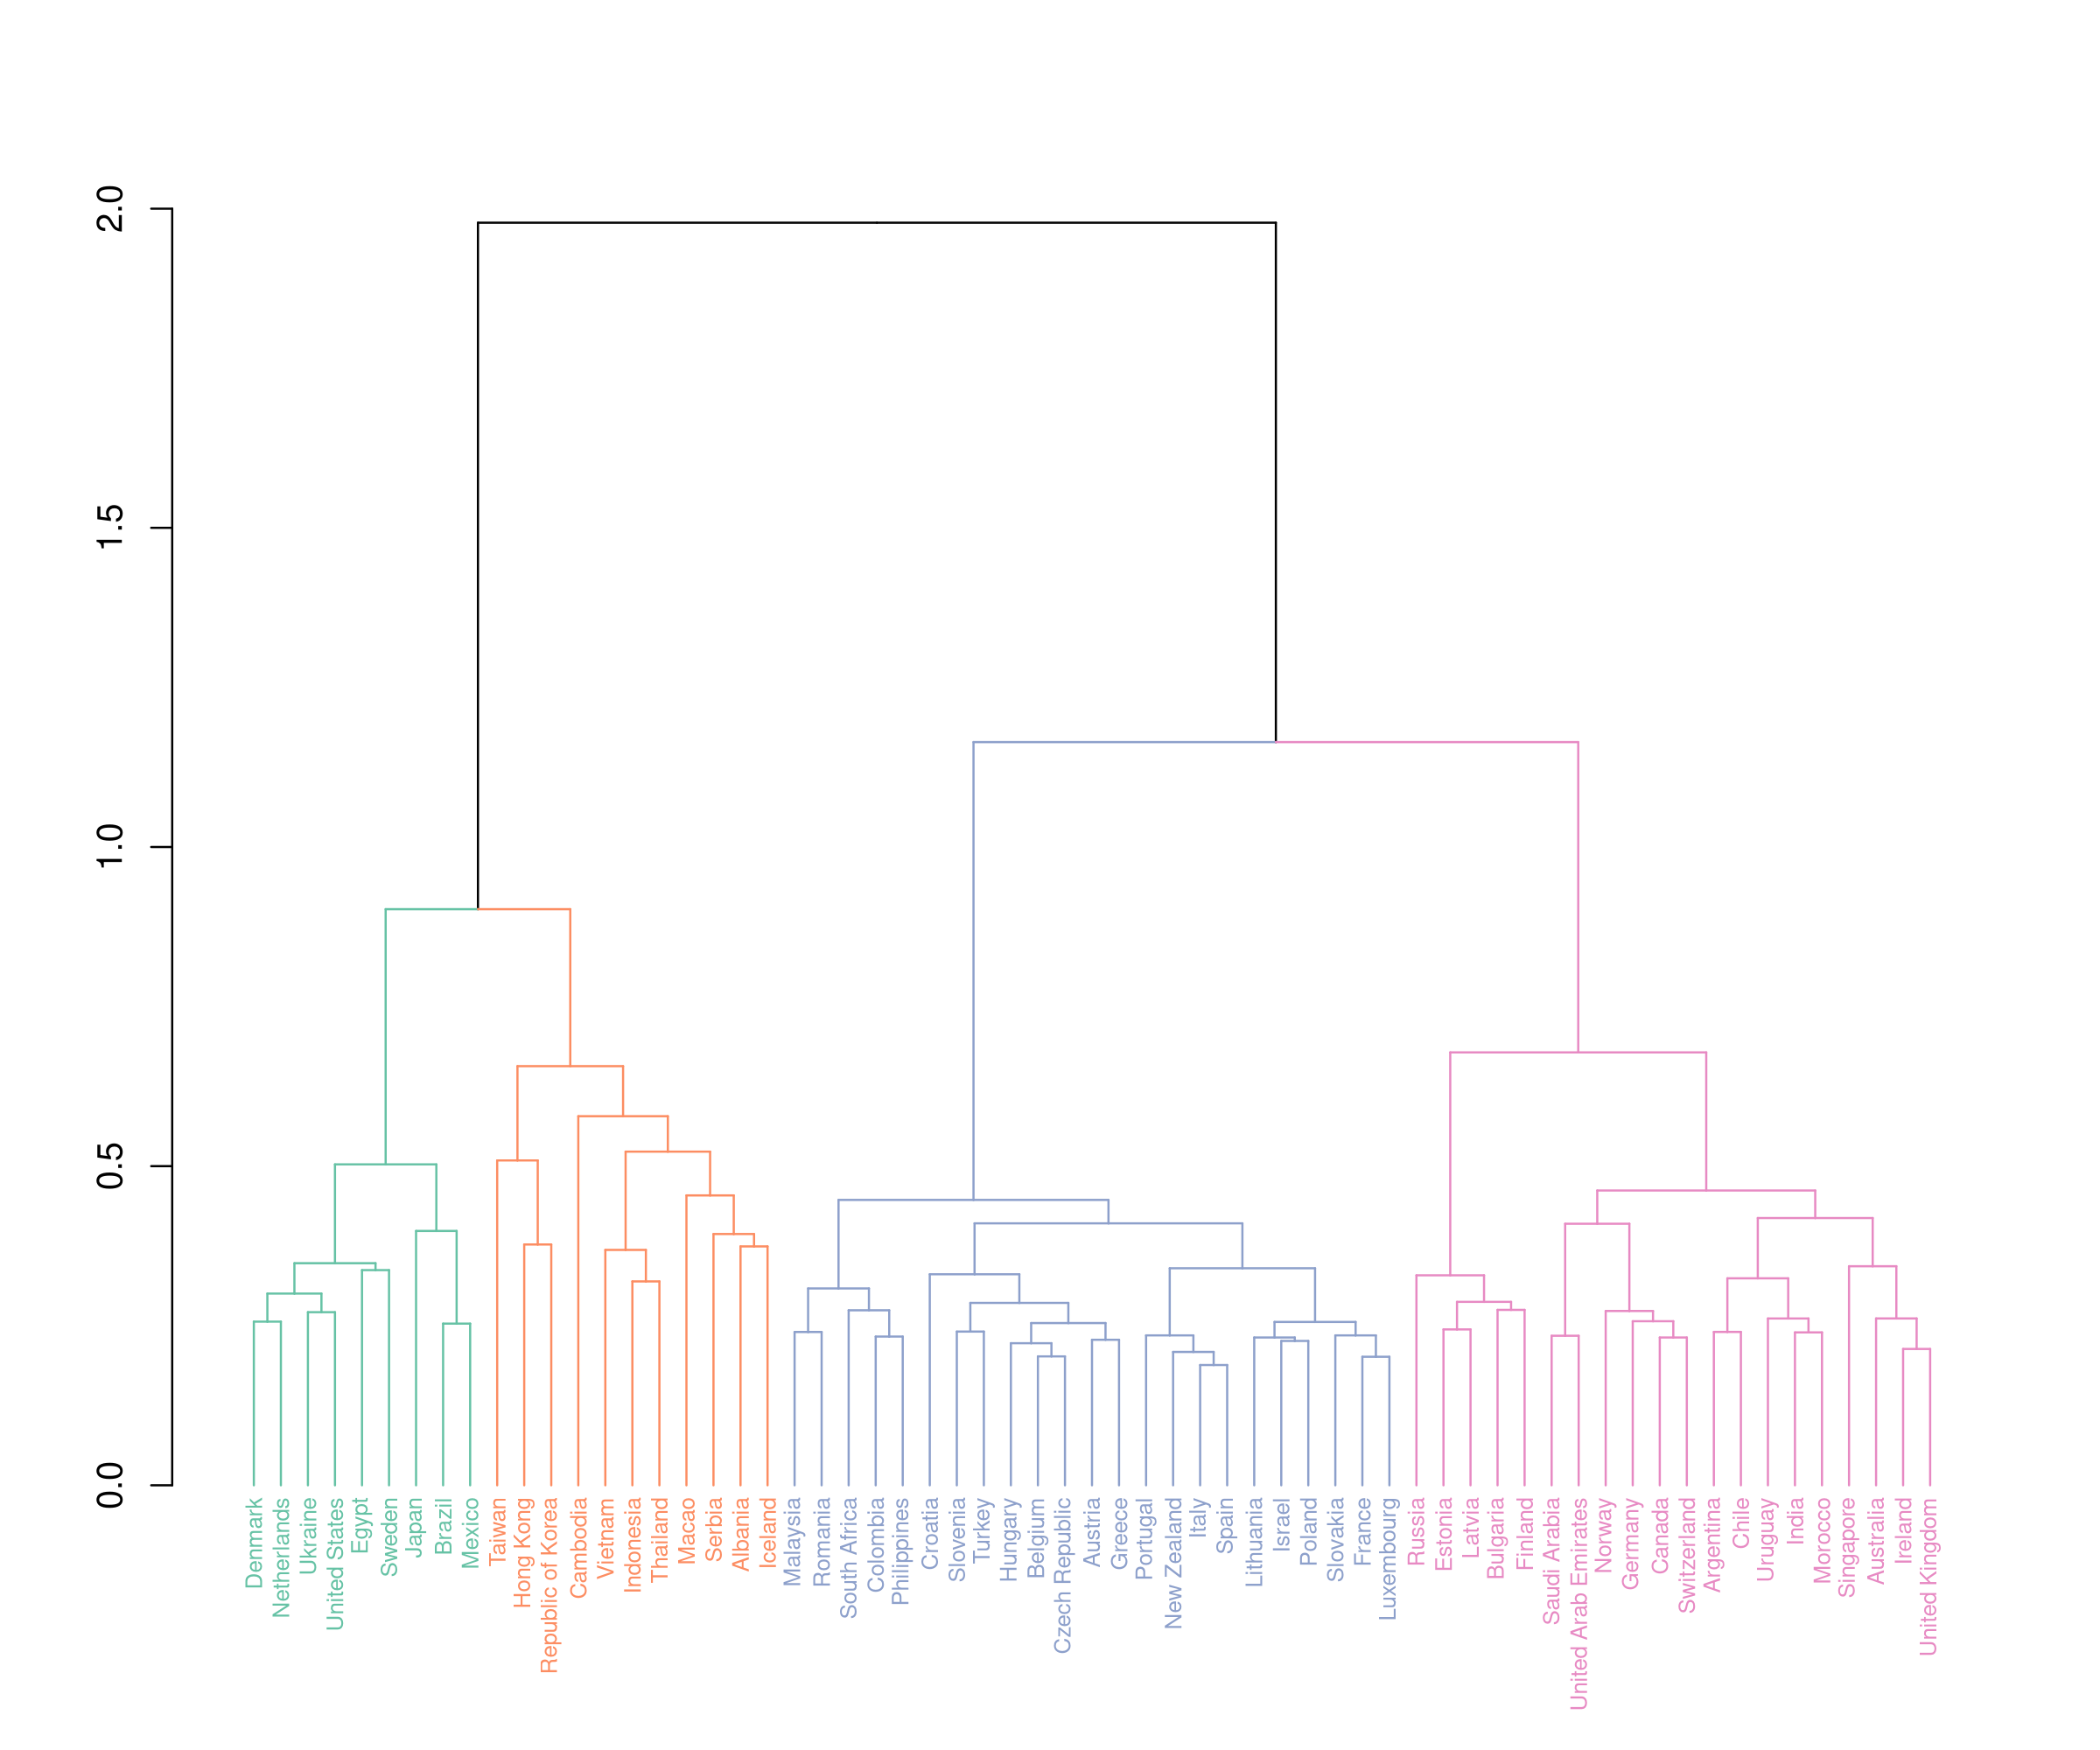
\includegraphics[width=\textwidth,trim={0cm 0 1.9cm 7cm},clip]{dendrogram}
  \caption{Dendrogram indicating four clusters of countries based on nine mobility and activity indicators}
  \label{fig:dend}
\end{figure}

We then plot the trends of activity changes as observed from Google location data, grouping these by cluster (\autoref{fig:act}).
Trends are shown by means of a generalized linear model estimated for each country.
Except in Cluster 1, which consists notably of South Korea, Hong Kong, Taiwan and Vietnam (countries with some of the best COVID-19 outcomes),
there was a significant downturn in work activities from mid-February to early April.
This decrease is as great as 75 percentage points in Clusters 2 and 3.
However, in Cluster 4 (e.g.\ United States, Brazil, Japan), it only reaches 50 percentage points.
The change in work activities can be seen as a partial indicator of lockdown policies or behavioral responses to the pandemic in each of the countries.
Transit activities similarly reduced in Clusters 2 and 3, but not as severely in Cluster 4.
Notably, in Cluster 1, transit stop activities dipped the lowest in South Korea compared to the other countries.
This outcome can be readily understood given that South Korea focused heavily on contact tracing to mitigate the spread of COVID-19 \trbcite{aum2020covid19,parkearly}.

Grocery shopping experienced a downturn in most countries. However, Clusters 1 and 4 show the smallest disruptions (a decline of about 20 percentage points).
The same trend is observed for retail activities.
However, in Cluster 4, this category had a more severe downturn (as many as 60 percentage points from the baseline), compared to grocery shopping.
This could be explained by policies keeping grocery stores open as essential services, while other retail outlets were shut.
Also, home activities (people staying in their places of residence) increased across all countries, peaking in April and then declining thereafter.
The change from baseline was greatest in Cluster 3 (generally over 50 percentage points), indicating that countries in this cluster stayed at home the most.
Furthermore, the peak for home activities occurs the latest in Cluster 3.

There are no discernible cluster-specific patterns for park activities for Clusters 1, 2 and 4 (as trends vary by country).
However, in Cluster 3, many countries observed a decline of up to 75 percentage points through April, followed by a large uptick.

\begin{figure}[h!]
  \centering
  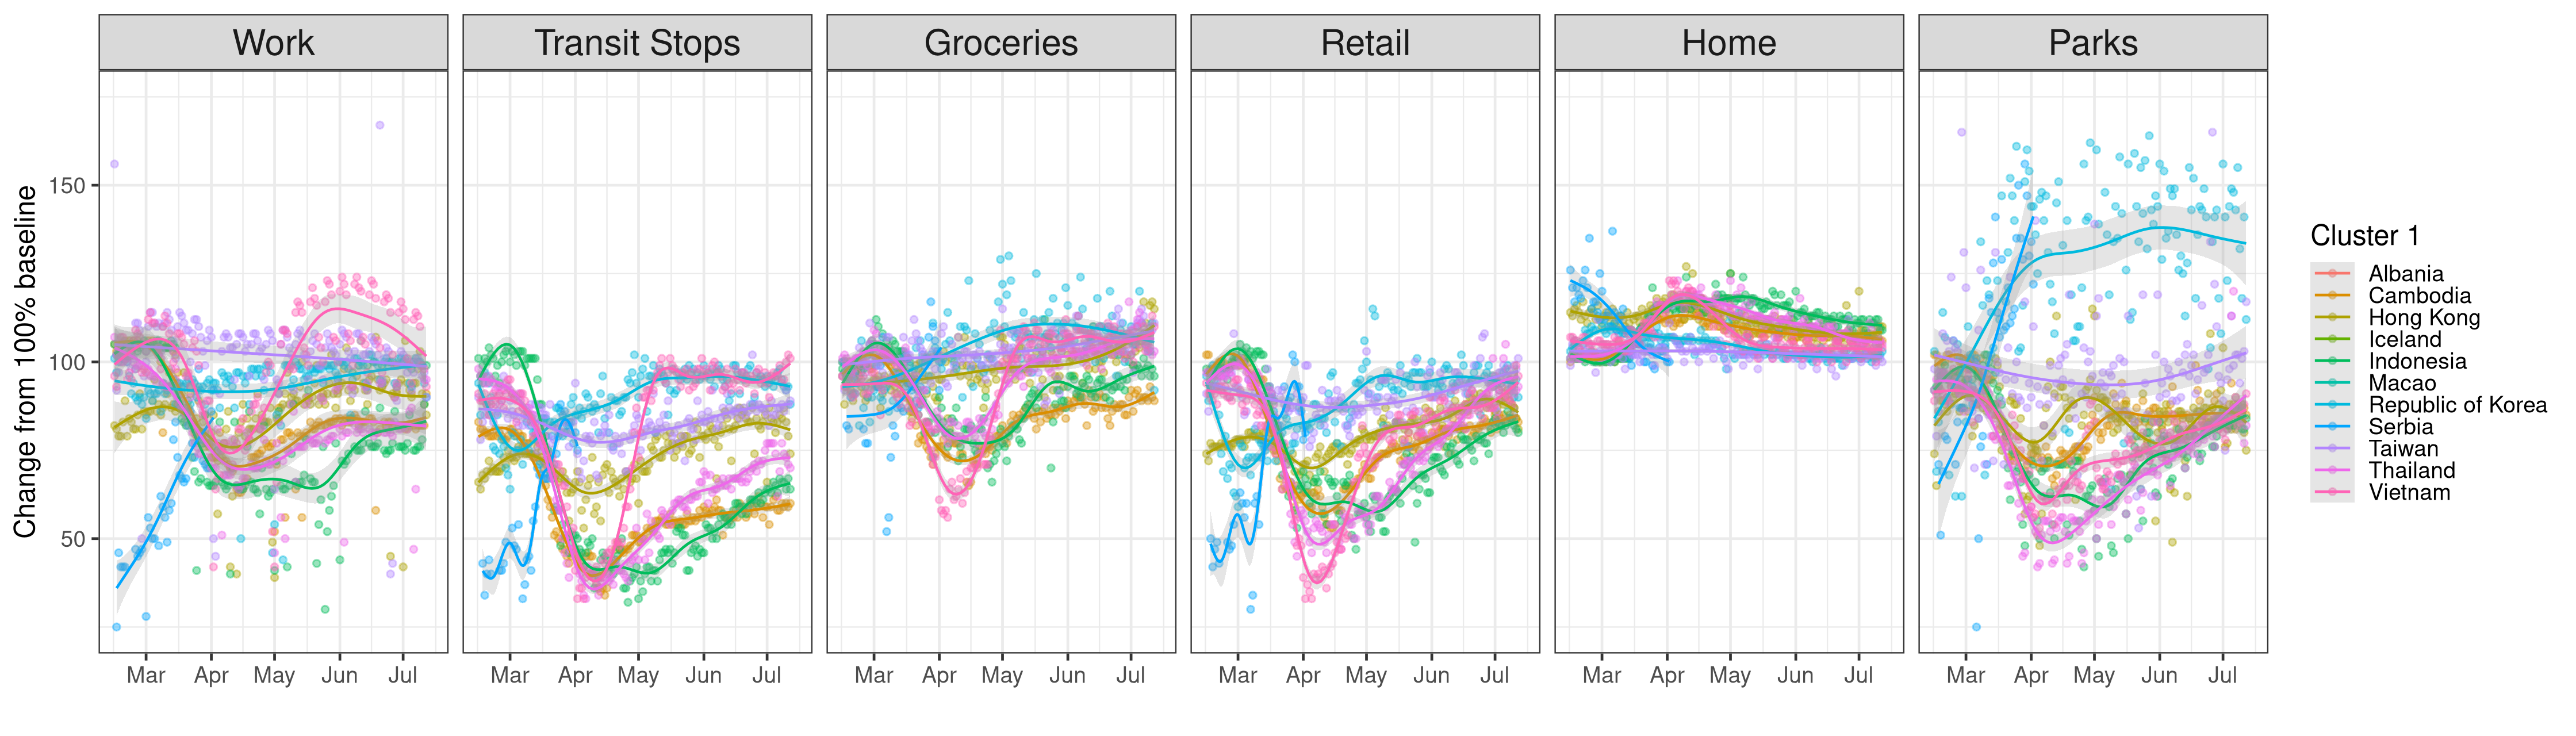
\includegraphics[width=\textwidth]{c1-activity}
  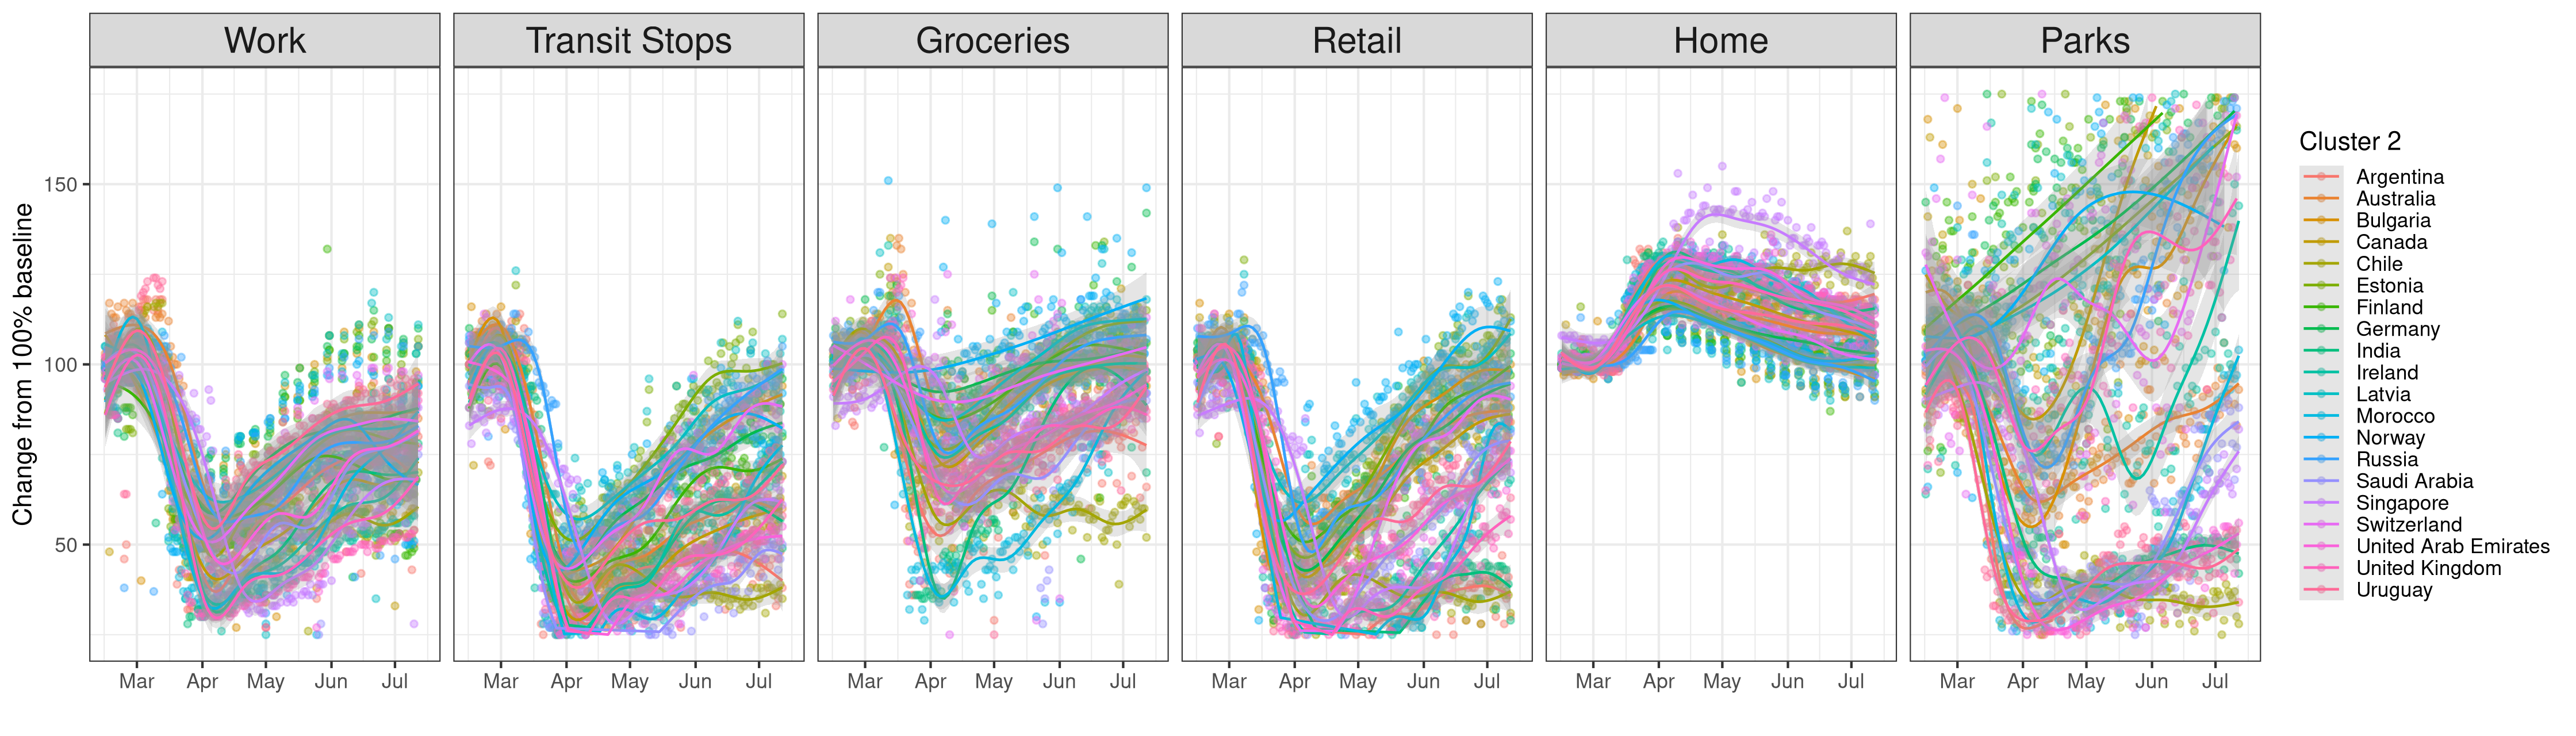
\includegraphics[width=\textwidth]{c2-activity}
  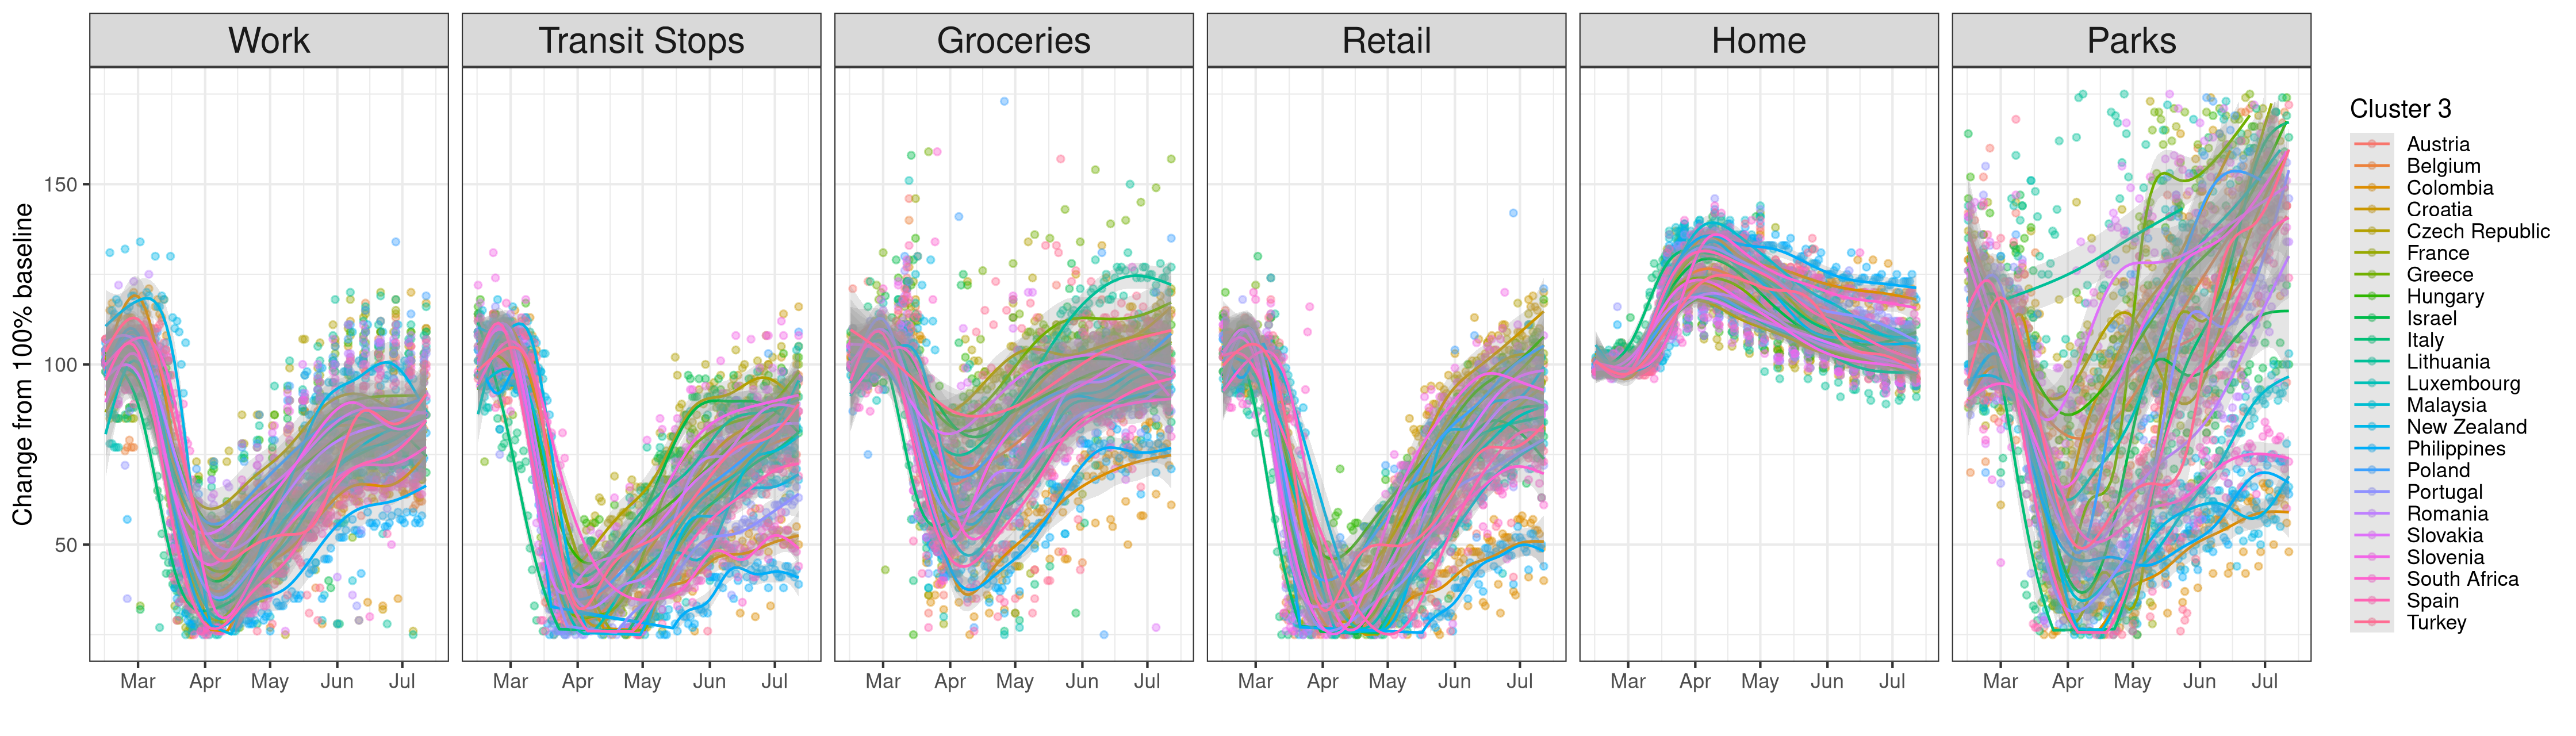
\includegraphics[width=\textwidth]{c3-activity}
  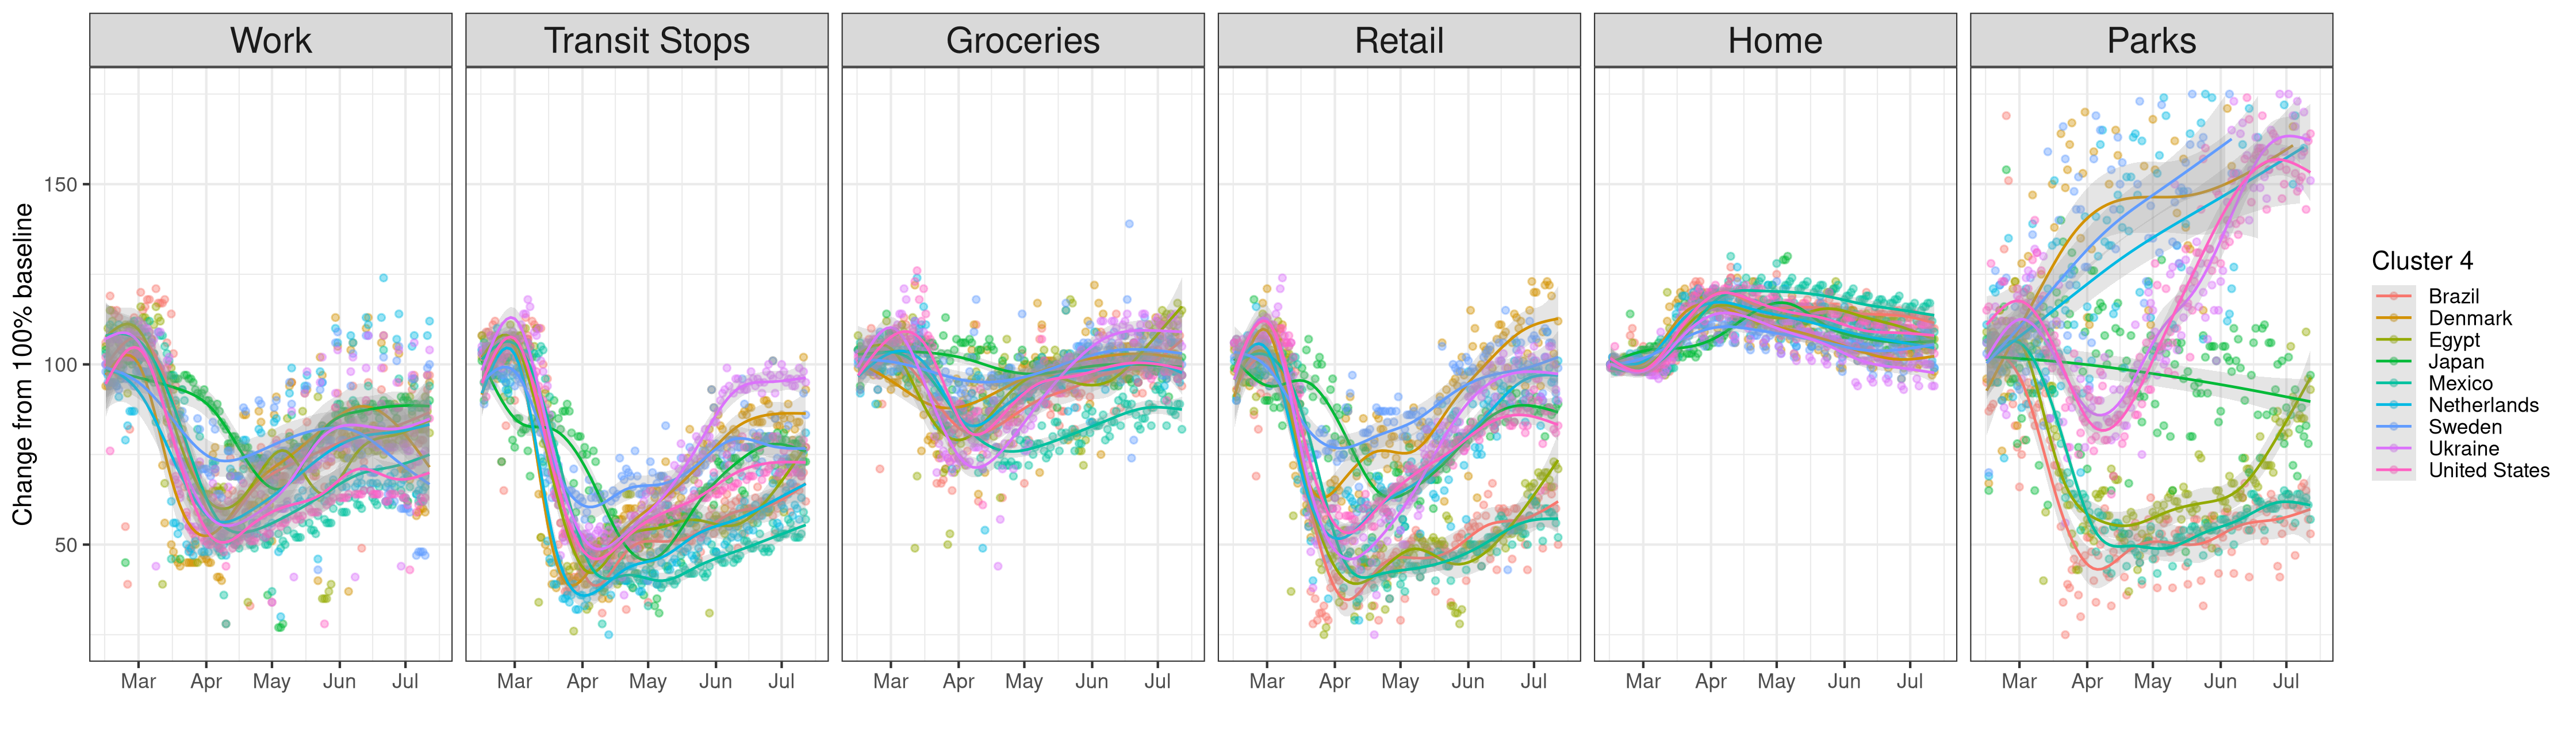
\includegraphics[width=\textwidth]{c4-activity}
  \caption{Activity changes from baseline (100\%) by cluster (Google dataset).  Trends are indicated using a generalized linear (GLM) fit for each country.}
  \label{fig:act}
\end{figure}


The driving, transit and walking activities observed from navigation via Apple devices do not distinctly vary among the clusters (\autoref{fig:mob}).
This could be explained by the fact that usual activities perhaps do not require navigation.
And also since Apple Maps users are not always representative of the population, it is less likely that changes in regular activities would be discernible from these data.

\begin{figure}[h!]
  \centering
  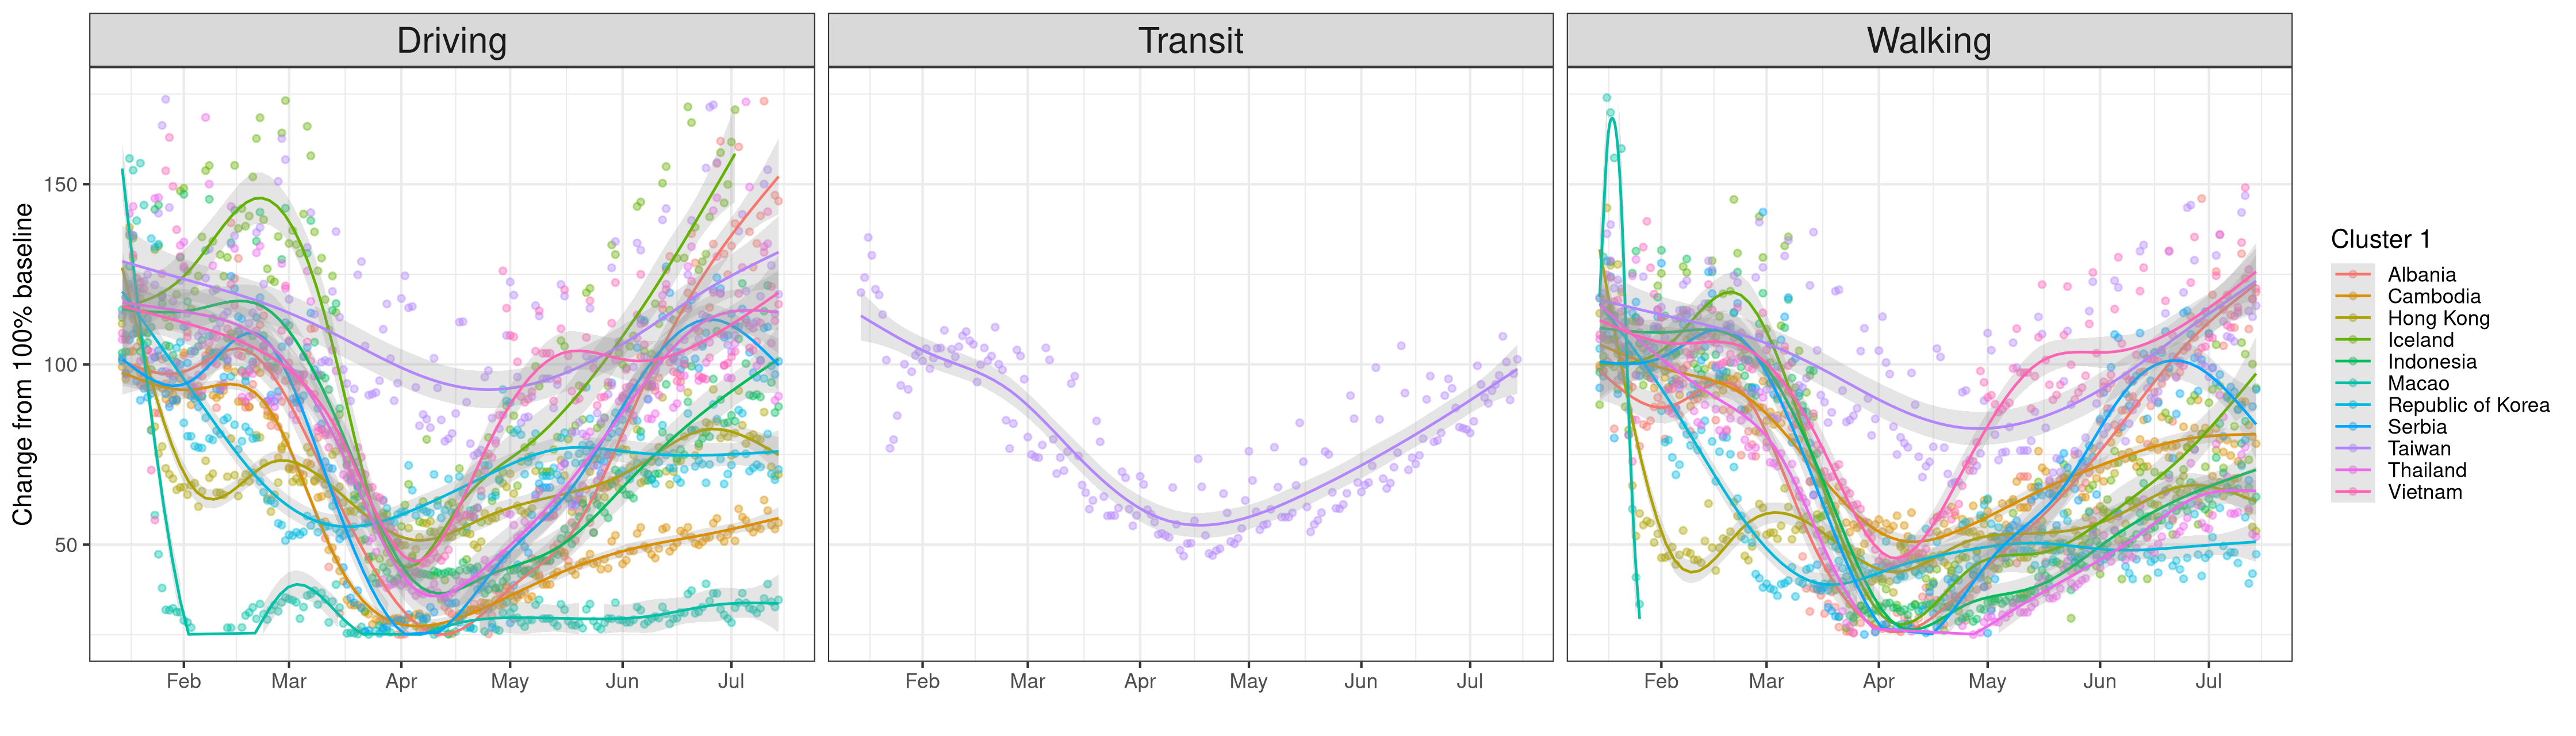
\includegraphics[width=.9\textwidth]{c1-mobility}
  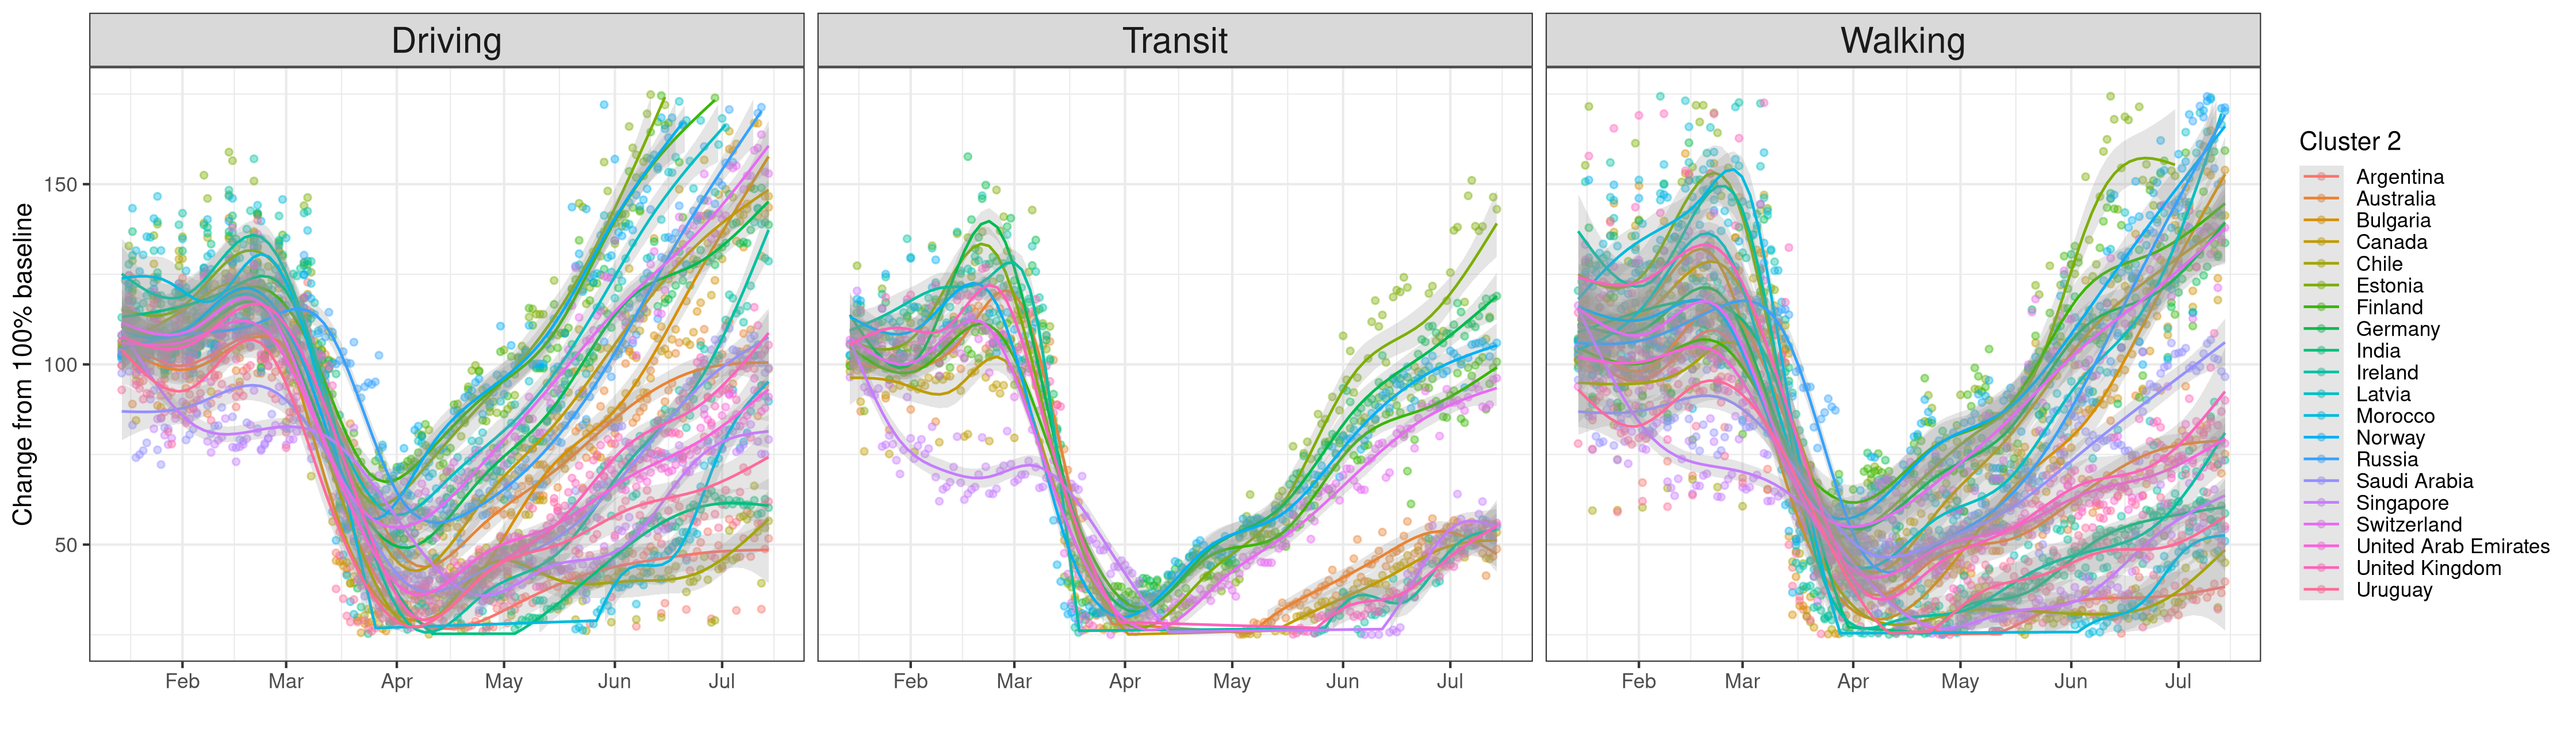
\includegraphics[width=.9\textwidth]{c2-mobility}
  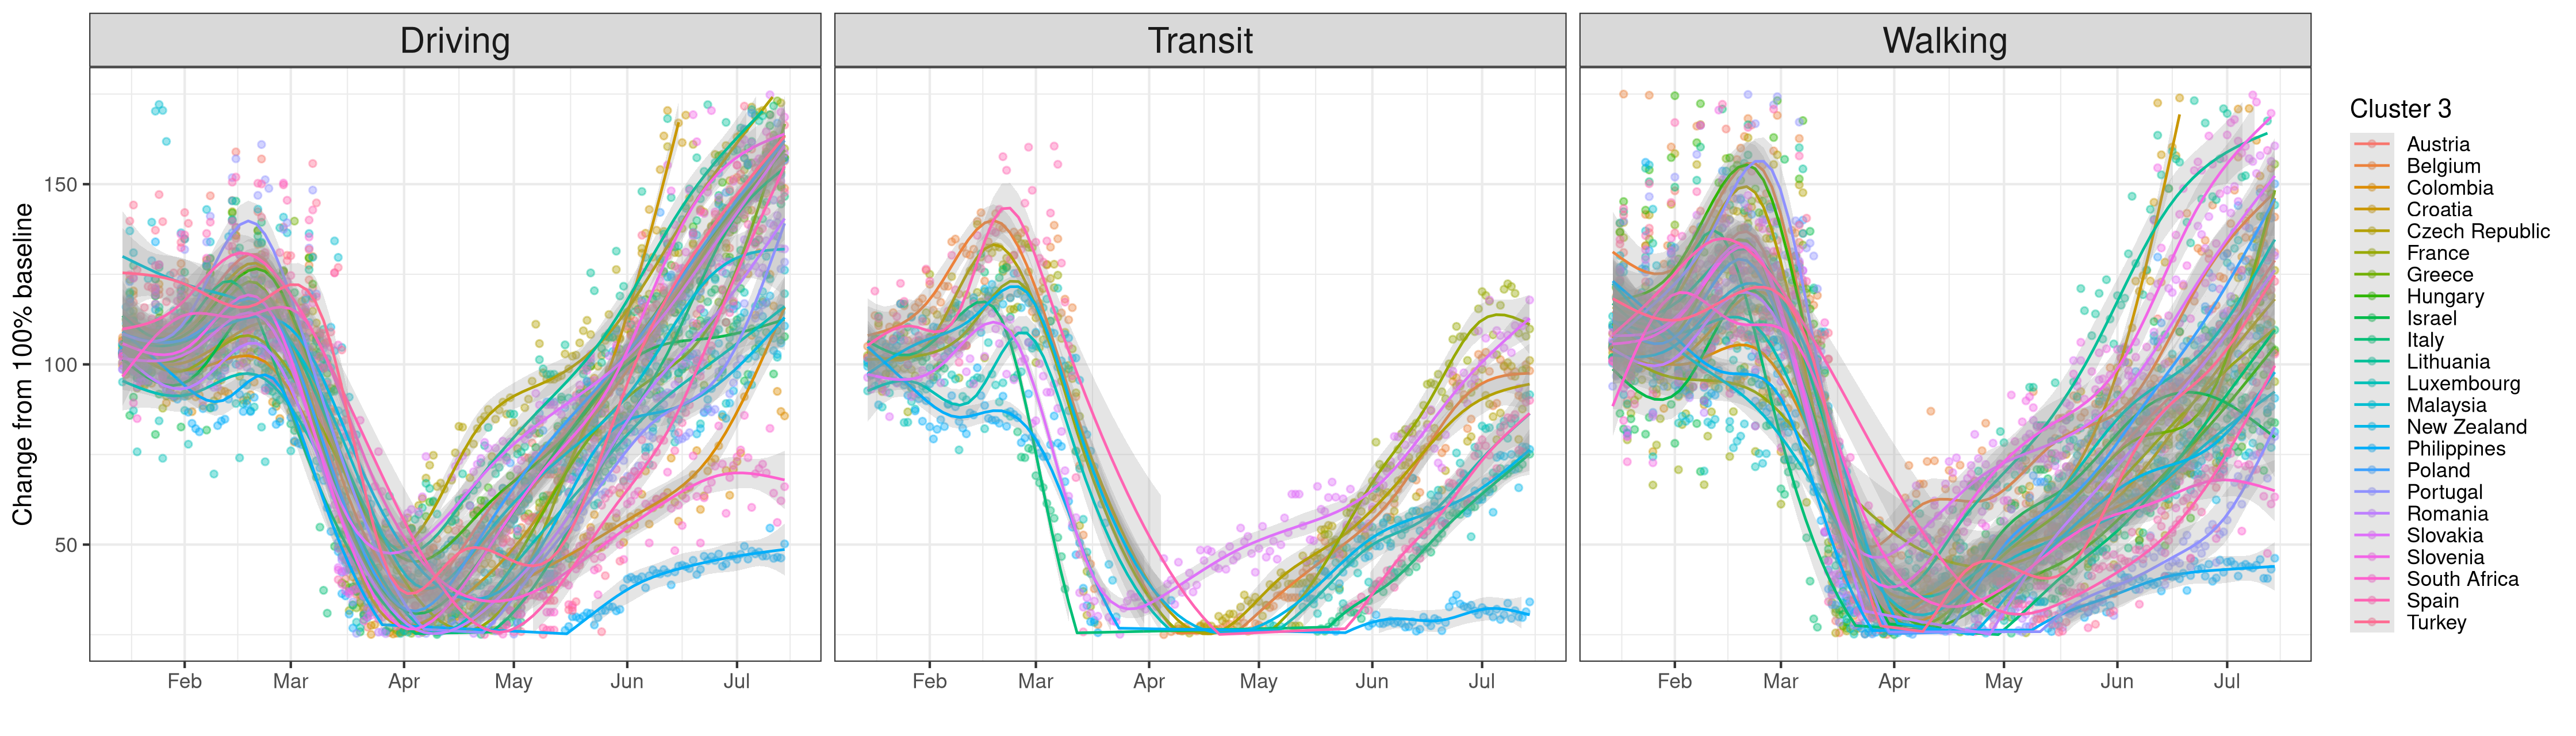
\includegraphics[width=.9\textwidth]{c3-mobility}
  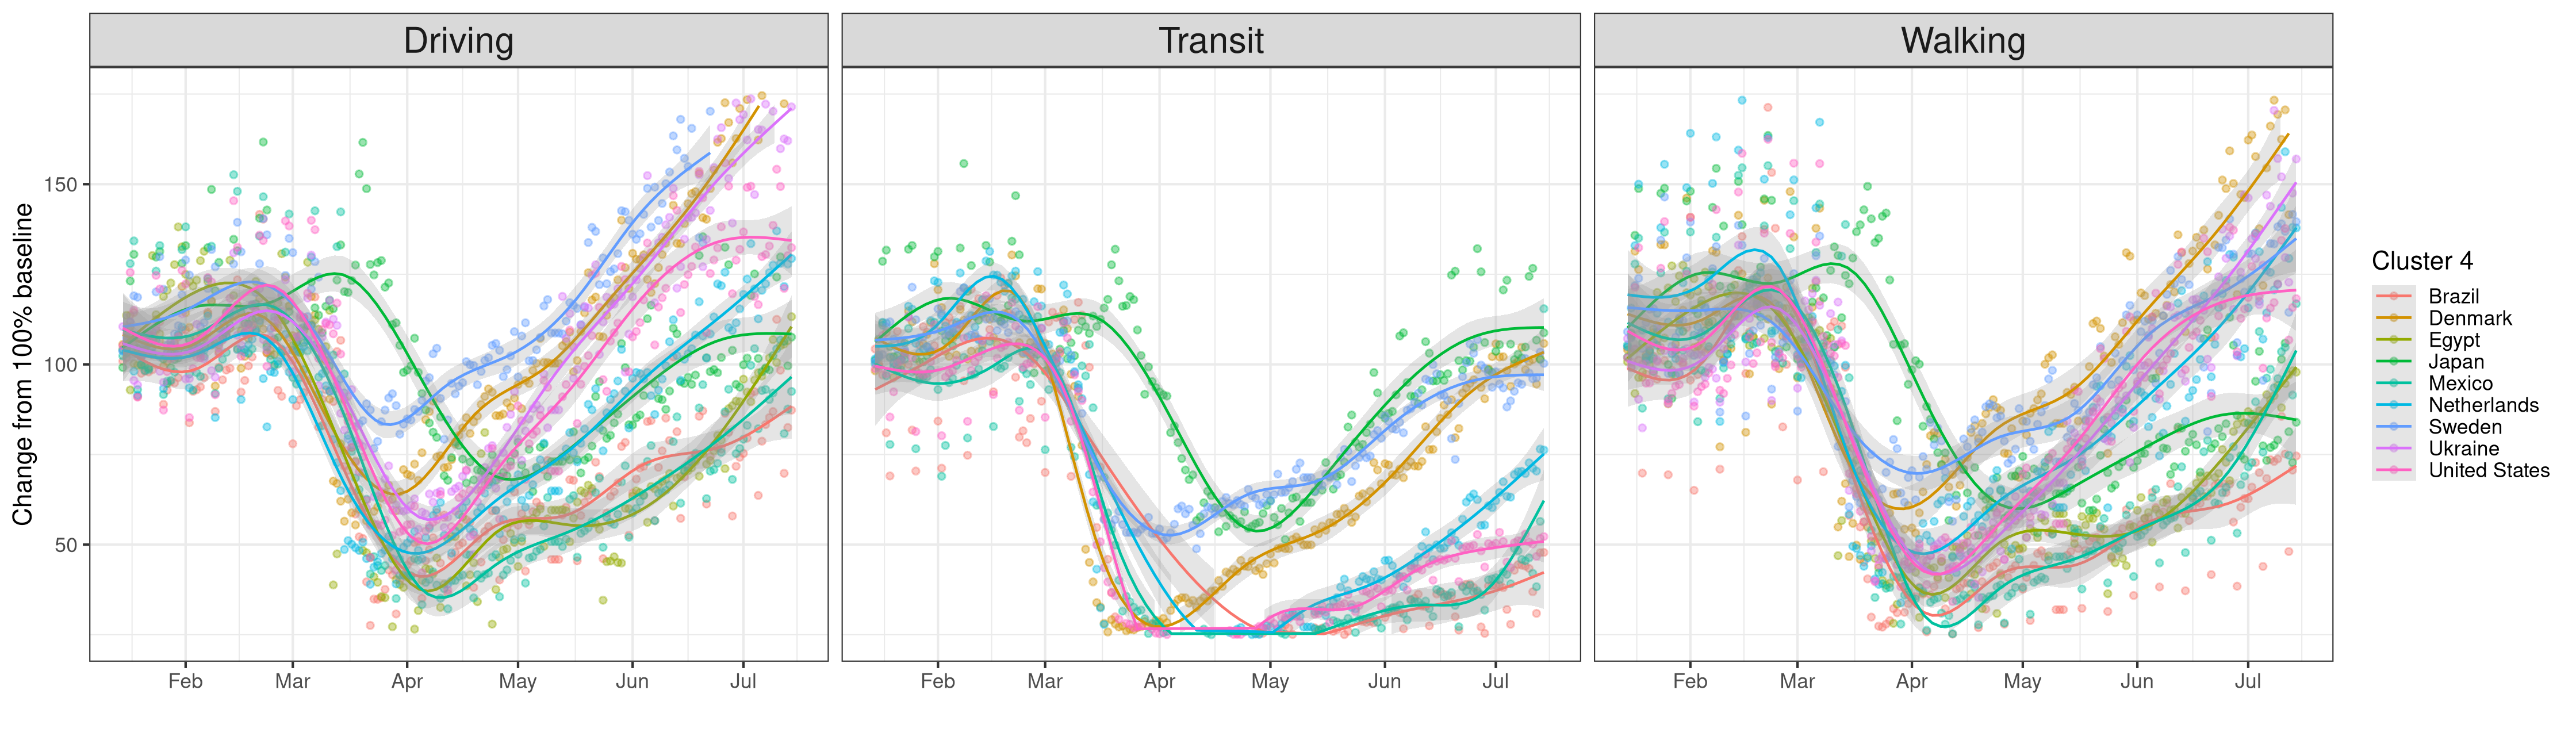
\includegraphics[width=.9\textwidth]{c4-mobility}
  \caption{Mobility changes from baseline (100\%) by cluster (Apple dataset). Trends are indicated using a generalized linear (GLM) fit for each country.}
  \label{fig:mob}
\end{figure}


We show the daily confirmed COVID-19 cases at the country level by cluster in \autoref{fig:cov} on a log-y scale.
Most of the countries in Cluster 1 have experienced a decrease in COVID-19 cases.
However, Serbia and Indonesia are outliers.
Given that the countries in this cluster had the least disruption in activities compared to other clusters, other exogenous factors are probably responsible for the favorable COVID-19 outcomes.
Clusters 2 and 3 were harder hit in the early weeks of the year, but indicate a downturn in COVID-19 infections from late March and early April.
These clusters had the most severe decreases in work and transit activities (and highest increases in home activities) from the baseline.
Clearly, there are few exceptions in each of these clusters, such as India in Cluster 2 and Colombia in Cluster 3.
Finally, in Cluster 4, most of the countries have been on an upward trajectory in recent weeks (except for Denmark).
In these countries, there is evidence of lockdowns being lifted too soon and perhaps less strict public health policies than elsewhere.
In terms of activities, this is one cluster where home activities showed the least disruption, which is an indicator of the aforementioned trend.

\begin{figure}[h!]
  \centering
  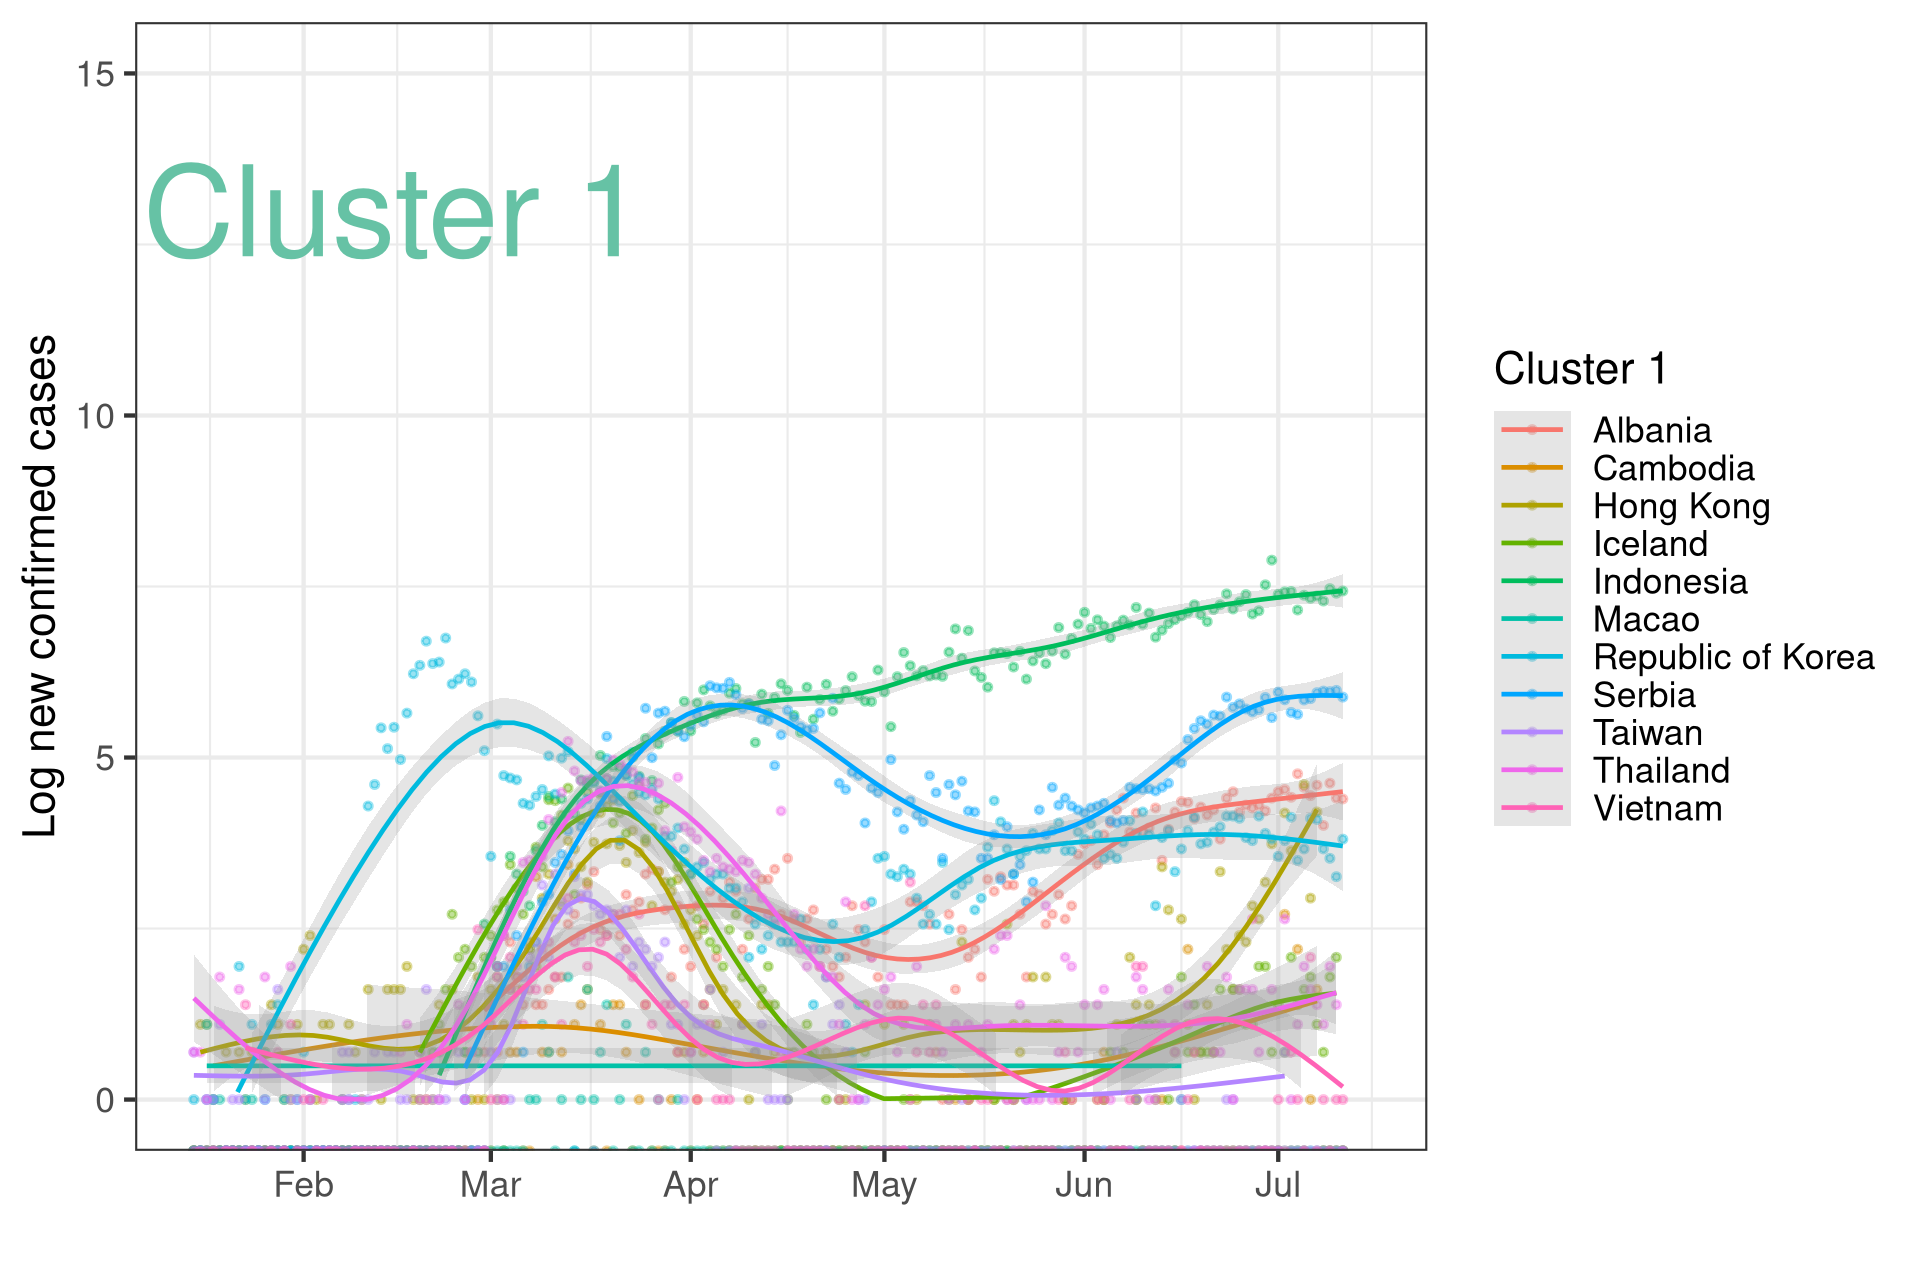
\includegraphics[width=.45\textwidth]{c1-cov}
  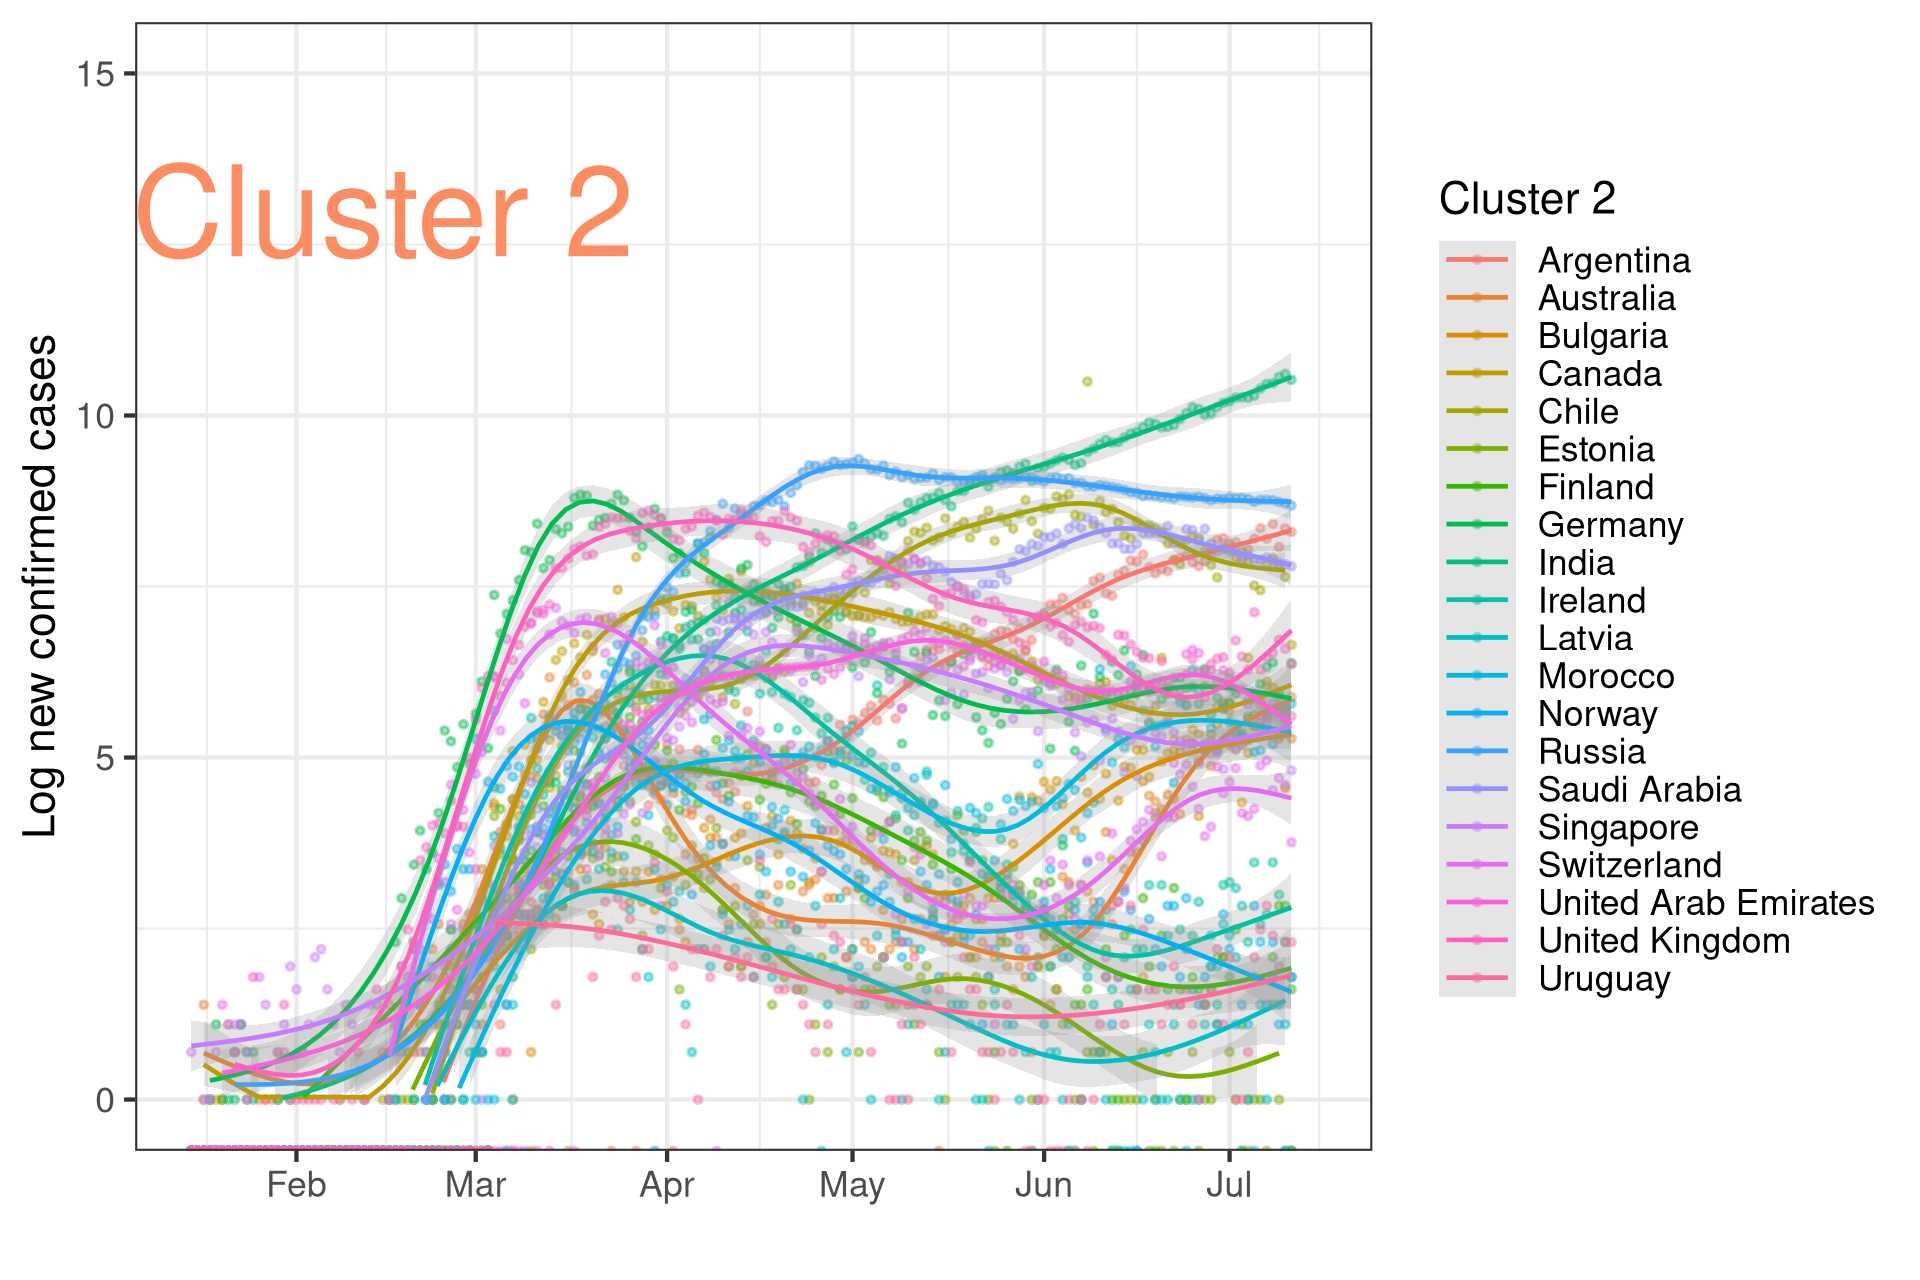
\includegraphics[width=.45\textwidth]{c2-cov}
  
  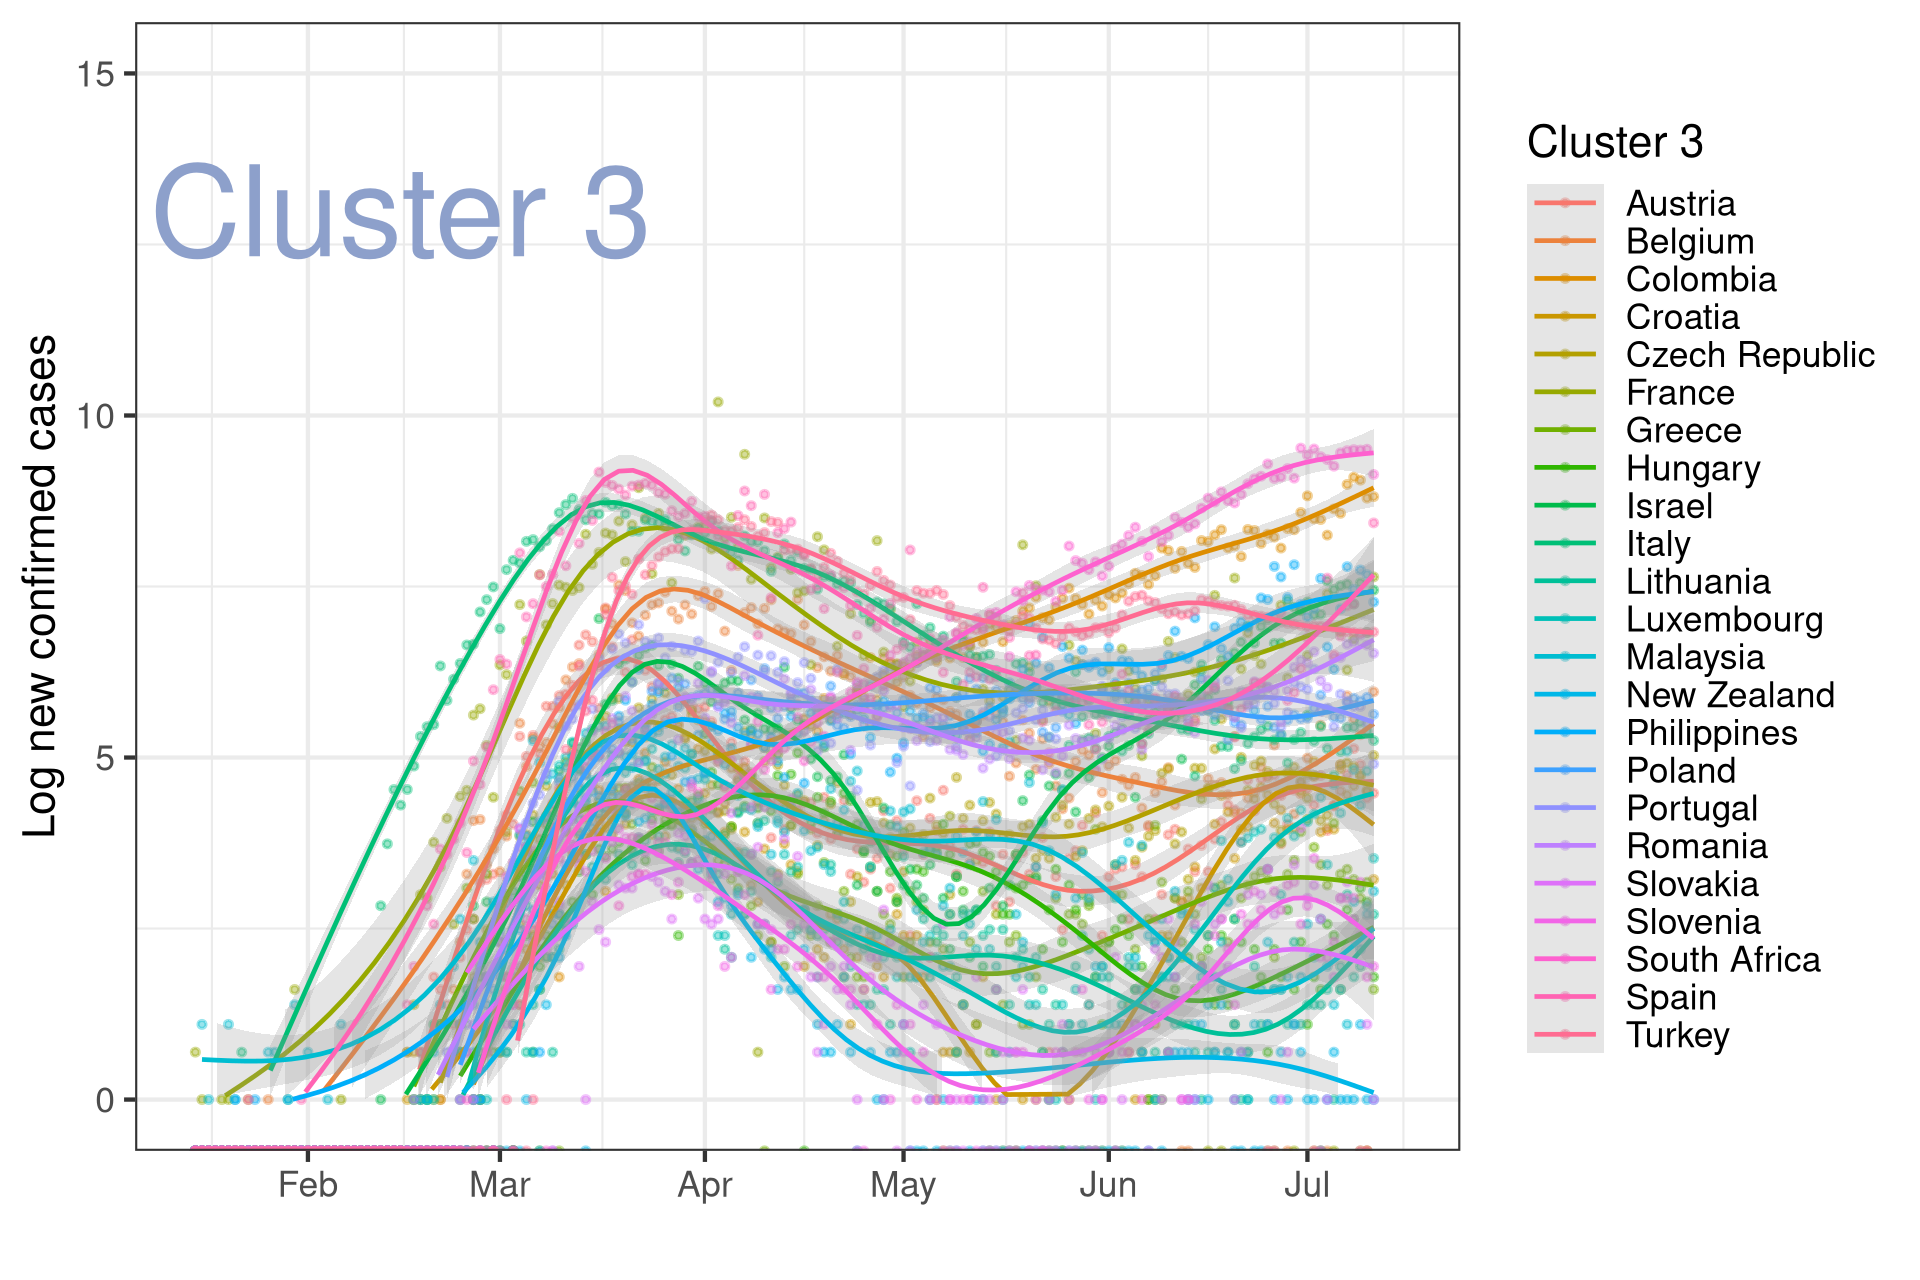
\includegraphics[width=.45\textwidth]{c3-cov}
  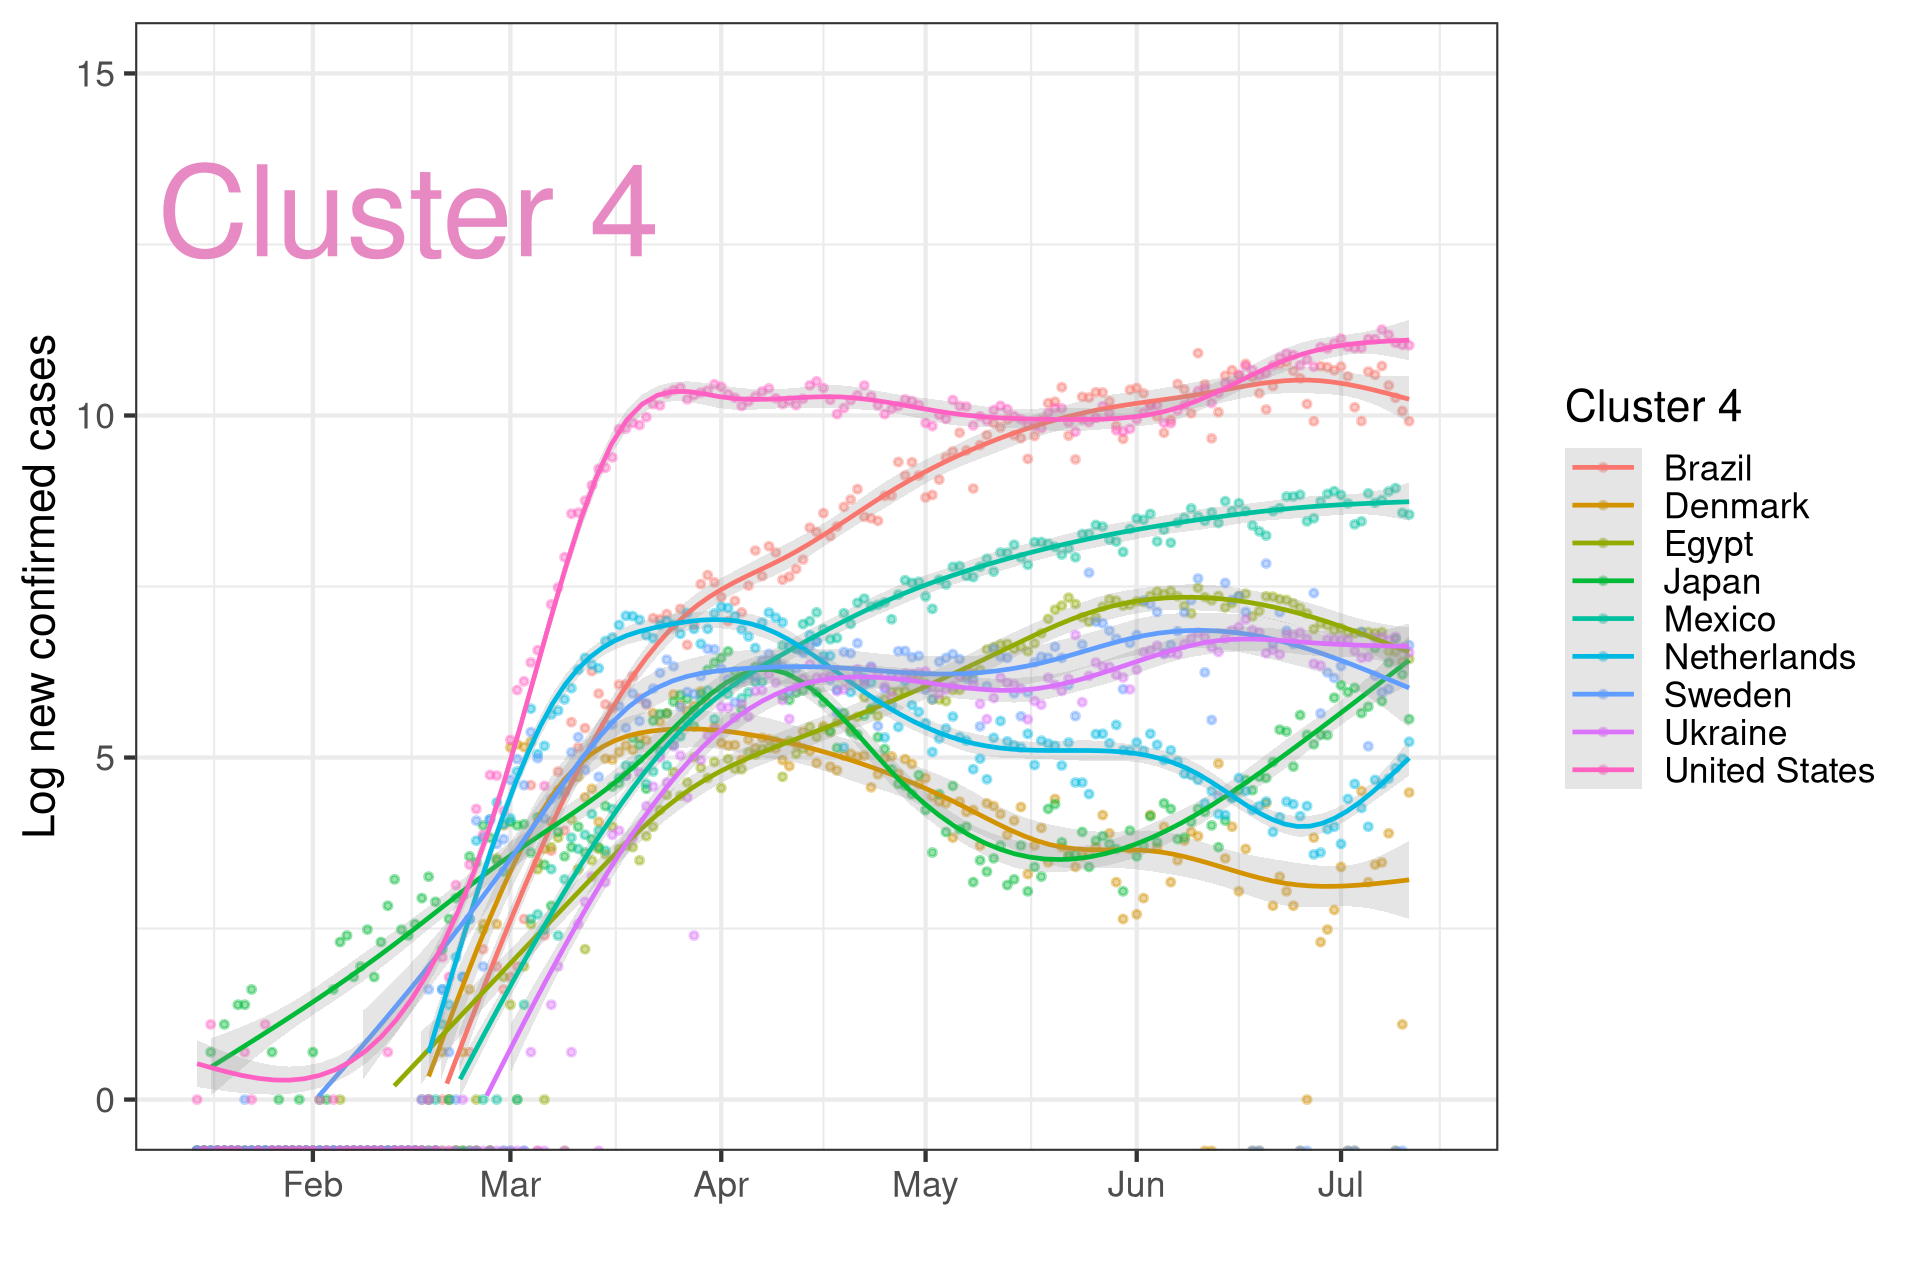
\includegraphics[width=.45\textwidth]{c4-cov}
  \caption{Daily confirmed COVID-19 cases for each of the clusters (log y-axis); Johns Hopkins dataset.}
  \label{fig:cov}
\end{figure}


\subsection{Expected results}
We plan to estimate country-level vector autoregression models (VARs), cluster-level panel VARs and a global VAR.
These models will enable us to explain how COVID-19 outcomes were impacted by changes across these activities.
They would also allow us to analyze how changes in one dimension would affect the other (using impulse response functions).
Other variables that can explain COVID-19 impacts (particularly interventions) will be included in these models as strictly exogenous variables.
Air passenger travel flows will also be incorporated as weights on weakly exogenous (foreign) variables in the global VAR model.
These would allow the inclusion of the effects of observations in other countries across these dimensions.


\section{Conclusion and future work}
We cluster the countries in our sample into four categories based on similar activity and mobility trends.
% By running the model with a different lag parameter for each country we attempted to estimate the optimal lag for each country.
% However, our VAR implementation fell short of producing statistically significant results.
Future work will focus on estimating VAR models for each of the countries, adding exogenous and weakly exogenous variables such as interventions and restrictions (social distancing orders, travel bans, etc.), as well as deterministic ones (country characteristics).
Subsequently, cluster-level VARs and a global VAR will be estimated.
These models will provide insights into the processes governing the changes in the endogenous variables (COVID-19 outcomes, activity and mobility trends), as well as potential forecasting capabilities.
The insights gained from these models would enable policy and decision makers plan efficiently for recovery from the current pandemic, as well as better prepare for future ones, by tailoring interventions relevant to the behavioral profiles of their respective countries.
%We also plan to substitute the number of new cases with a moving average for new COVID-19 cases which would produce more robust results.
 
% \section{Author Contribution Statement}
% The authors confirm contribution to the paper as follows: \\
% Study conception and design: \\
% Analysis and interpretation of results: \\
% Manuscript preparation:

%\section{Acknowledgment}

\bibliography{references.bib}
\bibliographystyle{trb}


\end{document}

%%% Local Variables:
%%% mode: latex
%%% TeX-master: t
%%% End:

